%%%%%%%%%%%%%%%%%%%%%%%%%%%%%%%%%%%%%%%%%%%%%%%%%%%%%%%%%%%%%%%%%%%%%%%%%%%%%%%%
%% Plantilla de memoria en LaTeX para la ETSIT - Universidad Rey Juan Carlos
%%
%% Por Gregorio Robles <grex arroba gsyc.urjc.es>
%%     Grupo de Sistemas y Comunicaciones
%%     Escuela Técnica Superior de Ingenieros de Telecomunicación
%%     Universidad Rey Juan Carlos
%% (muchas ideas tomadas de Internet, colegas del GSyC, antiguos alumnos...
%%  etc. Muchas gracias a todos)
%%
%% La última versión de esta plantilla está siempre disponible en:
%%     https://github.com/gregoriorobles/plantilla-memoria
%%
%% Para obtener PDF, ejecuta en la shell:
%%   make
%% (las imágenes deben ir en PNG o JPG)

%%%%%%%%%%%%%%%%%%%%%%%%%%%%%%%%%%%%%%%%%%%%%%%%%%%%%%%%%%%%%%%%%%%%%%%%%%%%%%%%

\documentclass[a4paper, 12pt]{book}
%\usepackage[T1]{fontenc}

\usepackage[a4paper, left=2.5cm, right=2.5cm, top=3cm, bottom=3cm]{geometry}
\usepackage{times}
\usepackage[utf8]{inputenc}
\usepackage[spanish]{babel} % Comenta esta línea si tu memoria es en inglés
\usepackage{url}
%\usepackage[dvipdfm]{graphicx}
\usepackage{graphicx}
\usepackage{subfigure}
\usepackage{float}  %% H para posicionar figuras
\usepackage[nottoc, notlot, notlof, notindex]{tocbibind} %% Opciones de índice
\usepackage{latexsym}  %% Logo LaTeX

\title{Memoria del Proyecto}
\author{Nombre del autor}

\renewcommand{\baselinestretch}{1.5}  %% Interlineado

\begin{document}

\renewcommand{\refname}{Bibliografía}  %% Renombrando
\renewcommand{\appendixname}{Apéndice}

%%%%%%%%%%%%%%%%%%%%%%%%%%%%%%%%%%%%%%%%%%%%%%%%%%%%%%%%%%%%%%%%%%%%%%%%%%%%%%%%
% PORTADA

\begin{titlepage}
\begin{center}
\includegraphics[scale=0.8]{img/URJ_logo_Color_POS.png}

\vspace{1.75cm}

\Large
GRADO EN INGENIERÍA EN SISTEMAS AUDIOVISUALES Y MULTIMEDIA

\vspace{0.4cm}

\large
Curso Académico 2021/2022

\vspace{0.8cm}

Trabajo Fin de Grado

\vspace{2.5cm}

\LARGE
IMPLEMENTACIÓN DE FUNCIONALIDADES EN LEARNINGML: RECONOCIMIENTO DE CONJUNTOS DE DATOS (DATASETS)

\vspace{3cm}

\large
Autor : Ignacio Rueda Rodríguez \\
Tutor : Dr. Gregorio Robles Martínez \\
Co-tutor : Juan David Rodríguez García
\end{center}
\end{titlepage}

\newpage
\mbox{}
\thispagestyle{empty} % para que no se numere esta pagina


%%%%%%%%%%%%%%%%%%%%%%%%%%%%%%%%%%%%%%%%%%%%%%%%%%%%%%%%%%%%%%%%%%%%%%%%%%%%%%%%
%%%% Para firmar
\clearpage
\pagenumbering{gobble}
\chapter*{}

\vspace{-4cm}
\begin{center}
\LARGE
\textbf{Trabajo Fin de Grado}

\vspace{1cm}
\large
Implementación de Funcionalidades en LearningML: Reconocimiento de Conjuntos de Datos (Datasets)

\vspace{1cm}
\large
\textbf{Autor :} Ignacio Rueda Rodríguez \\
\textbf{Tutor :} Dr. Gregorio Robles Martínez \\
\textbf{Co-tutor :} Juan David Rodríguez García

\end{center}

\vspace{1cm}
La defensa del presente Proyecto Fin de Carrera se realizó el día \qquad$\;\,$ de \qquad\qquad\qquad\qquad \newline de 2022, siendo calificada por el siguiente tribunal:


\vspace{0.5cm}
\textbf{Presidente:}

\vspace{1.2cm}
\textbf{Secretario:}

\vspace{1.2cm}
\textbf{Vocal:}


\vspace{1.2cm}
y habiendo obtenido la siguiente calificación:

\vspace{1cm}
\textbf{Calificación:}


\vspace{1cm}
\begin{flushright}
Fuenlabrada, a \qquad$\;\,$ de \qquad\qquad\qquad\qquad de 2022
\end{flushright}

%%%%%%%%%%%%%%%%%%%%%%%%%%%%%%%%%%%%%%%%%%%%%%%%%%%%%%%%%%%%%%%%%%%%%%%%%%%%%%%%
%%%% Dedicatoria

\chapter*{}
\pagenumbering{Roman} % para comenzar la numeracion de paginas en numeros romanos
\begin{flushright}
\textit{Dedicado a \\
mi familia, abuelos y amigos}
\end{flushright}

%%%%%%%%%%%%%%%%%%%%%%%%%%%%%%%%%%%%%%%%%%%%%%%%%%%%%%%%%%%%%%%%%%%%%%%%%%%%%%%%
%%%% Agradecimientos

\chapter*{Agradecimientos}
%\addcontentsline{toc}{chapter}{Agradecimientos} % si queremos que aparezca en el índice
\markboth{AGRADECIMIENTOS}{AGRADECIMIENTOS} % encabezado 

Aquí vienen los agradecimientos\ldots Aunque está bien acordarse de la pareja, no hay que olvidarse de dar las gracias a tu madre, que aunque a veces no lo parezca disfrutará tanto de tus logros como tú\ldots 
Además, la pareja quizás no sea para siempre, pero tu madre sí.



%%%%%%%%%%%%%%%%%%%%%%%%%%%%%%%%%%%%%%%%%%%%%%%%%%%%%%%%%%%%%%%%%%%%%%%%%%%%%%%%
%%%% Resumen

\chapter*{Resumen}
%\addcontentsline{toc}{chapter}{Resumen} % si queremos que aparezca en el índice
\markboth{RESUMEN}{RESUMEN} % encabezado

El objetivo de este proyecto consiste en añadir una nueva funcionalidad para el reconocimiento de conjuntos de datos a la aplicación web \texttt{LearningML}, que ya reconoce imágenes y textos. Los conjuntos de datos son una colección de datos tabulados, estos datos pueden ser numéricos y categóricos.

\texttt{LearningML} es una aplicación web que tiene como objetivo ayudar a los profesores de secundaria a explicar de una manera sencilla y visual el machine learning y para fomentar las habilidades de pensamiento computacional en alumnos de entre 10 y 16 años.

\texttt{LearningML} está creada en angular, que es un entorno de trabajo que utiliza HTML y CSS para la creación de aplicaciones web y utiliza TypeScript para implementar la funcionalidad de las aplicaciones web. Para llevar a cabo este proyecto ha sido necesario crear un nuevo servicio y un nuevo componente además de modificar algunos componentes y servicios, y crear distintas funciones pero siguiendo la dinámica de lo ya creado.

%%%%%%%%%%%%%%%%%%%%%%%%%%%%%%%%%%%%%%%%%%%%%%%%%%%%%%%%%%%%%%%%%%%%%%%%%%%%%%%%
%%%% Resumen en inglés

\chapter*{Summary}
%\addcontentsline{toc}{chapter}{Summary} % si queremos que aparezca en el índice
\markboth{SUMMARY}{SUMMARY} % encabezado

The goal of this project consists of adding new functionality for the recognition of datasets to the \texttt{LearningML} web application, which already recognises images and text. Datasets are a collection of tabulated data, these data can be numerical and categorical.

\texttt{LearningML} is a web application that aims to help secondary school teachers explain machine learning in a simple and visual way and to foster computational thinking skills in students aged 10-16.

\texttt{LearningML} is based on Angular, which is a framework that uses HTML and CSS to create web applications and uses TypeScript to implement the functionality of the web application. To carry out this project it has been necessary to create a new service and a new component, as well as to modify some components and services, and to create different functions but following the dynamics of what has already been created.


%%%%%%%%%%%%%%%%%%%%%%%%%%%%%%%%%%%%%%%%%%%%%%%%%%%%%%%%%%%%%%%%%%%%%%%%%%%%%%%%
%%%%%%%%%%%%%%%%%%%%%%%%%%%%%%%%%%%%%%%%%%%%%%%%%%%%%%%%%%%%%%%%%%%%%%%%%%%%%%%%
% ÍNDICES %
%%%%%%%%%%%%%%%%%%%%%%%%%%%%%%%%%%%%%%%%%%%%%%%%%%%%%%%%%%%%%%%%%%%%%%%%%%%%%%%%

% Las buenas noticias es que los índices se generan automáticamente.
% Lo único que tienes que hacer es elegir cuáles quieren que se generen,
% y comentar/descomentar esa instrucción de LaTeX.

%%%% Índice de contenidos
\tableofcontents 
%%%% Índice de figuras
\cleardoublepage
%\addcontentsline{toc}{chapter}{Lista de figuras} % para que aparezca en el indice de contenidos
\listoffigures % indice de figuras
%%%% Índice de tablas
%\cleardoublepage
%\addcontentsline{toc}{chapter}{Lista de tablas} % para que aparezca en el indice de contenidos
%\listoftables % indice de tablas


%%%%%%%%%%%%%%%%%%%%%%%%%%%%%%%%%%%%%%%%%%%%%%%%%%%%%%%%%%%%%%%%%%%%%%%%%%%%%%%%
%%%%%%%%%%%%%%%%%%%%%%%%%%%%%%%%%%%%%%%%%%%%%%%%%%%%%%%%%%%%%%%%%%%%%%%%%%%%%%%%
% INTRODUCCIÓN %
%%%%%%%%%%%%%%%%%%%%%%%%%%%%%%%%%%%%%%%%%%%%%%%%%%%%%%%%%%%%%%%%%%%%%%%%%%%%%%%%

\cleardoublepage
\chapter{Introducción}
\label{sec:intro} % etiqueta para poder referenciar luego en el texto con ~\ref{sec:intro}
\pagenumbering{arabic} % para empezar la numeración de página con números

En la actualidad, se generan una cantidad inmensa de datos digitales, tantos que se han multiplicado por más de treinta en la última década, pasando de dos zetabytes en 2010 a 64 zetabytes en 2020 y esta cantidad seguirá aumentando de forma exponencial~\cite{Pagina_de_Datos}. 
El problema es el procesamiento de los datos, ya que debido a su complejidad los humanos no somos capaces de extraer información útil de tal cantidad de datos en un tiempo aceptable, para ello se utiliza la inteligencia artificial. 
El machine learning es una de las ramas de la inteligencia artificial que se usa para el procesamiento y análisis de los datos, puesto que es capaz de analizar una gran cantidad de datos de manera eficiente y transformarlos en información más sencilla, legible y fácil de analizar por los humanos además de aportar muchas utilidades a partir de los datos que se generan, como puede ser anuncios personalizados en internet~\cite{rouhiainen2018inteligencia}.

Debido al aumento del uso de la inteligencia artificial y del aprendizaje automático, Juan David Rodríguez García decide crear la aplicación web \texttt{LearningML} dado que es un apasionado de la programación y al ser docente cree  que la introducción de contenidos de inteligencia artificial en la escuela a través de proyectos prácticos es el camino a seguir para educar ciudadanos conscientes y críticos, para despertar vocaciones entre los jóvenes y para fomentar las habilidades de pensamiento computacional. Por eso fue evaluada por estudiantes de 10 a 16 años mostrando su utilidad para aprender conceptos de inteligencia artificial y machine learning~\cite{Pagina_de_LearningML}.

\texttt{LearningML}\footnote{https://learningml.org/editor/} es una aplicación web dirigida al aprendizaje automático supervisado, una de las técnicas de IA más exitosas que se encuentra en la base de casi todas las aplicaciones actuales de IA y con la que se pretende cubrir la falta de herramientas para la enseñanza práctica de la inteligencia artificial. 
Es una herramienta que permite la enseñanza del aprendizaje automático de una forma sencilla haciendo que el reconocimiento de imágenes o el reconocimiento de textos se pueda hacer y observar de una manera sencilla y fácil de ver. 
Hace uso de los algoritmos de redes neuronales y KNN, permite descargar el modelo creado en un archivo JSON para poder usar ese modelo en otro momento y no tener que crear de nuevo el modelo, tiene la opción de registrarse para poder guardar los modelos en la nube y permite crear un modelo en Scratch y utilizarlo en \texttt{LearningML}. Scratch es un entorno de programación que aprovecha los avances en el diseño de interfaces para hacer que la programación sea atractiva y accesible para todo aquel que se enfrente por primera vez a programar, es el entorno utilizado en institutos y colegios para empezar a enseñar la programación a los adolescentes.

Este proyecto consiste en la integración de un nuevo tipo de reconocimiento: el reconocimiento de conjuntos de datos, siguiendo la dinámica de lo ya creado y en el que se crea un componente, un servicio y se modifican varios componentes para poder llevar a cabo la implementación de la nueva funcionalidad. 
Los conjuntos de datos es una de las formas de almacenar todos los datos que se generan y por eso creo que es interesante que se disponga de este tipo de reconocimiento. Para hacer reconocimento de conjuntos de datos 


\section{Estructura de la memoria}
\label{sec:estructura}

La memoria de este trabajo se divide en seis capítulos resumidos a continuación:

\begin{itemize}
  \item[•] \textbf{Capítulo 1: Introducción.} Se explica el contexto en el que se ha desarrollado, se hace una breve explicación de qué es, para qué se usa y cuál es el objetivo de la aplicación web \texttt{LearningML}, y la estructura de la memoria.
  
  \item[•] \textbf{Capítulo 2: Objetivos.} Se describen tanto el objetivo principal como los objetivos específicos y la planificación temporal del proyecto.
  
  \item[•] \textbf{Capítulo 3: Estado del arte.} Se explican cada una de las tecnologías utilizadas en el desarrollo del proyecto.
  
  \item[•] \textbf{Capítulo 4: Diseño e implementación.} Se explica detalladamente la arquitectura de \texttt{LearningML} y los cambios realizados sobre la arquitectura, así como el desarrollo e implementación de la nueva funcionalidad para reconocer conjuntos de datos.
  
  \item[•] \textbf{Capítulo 5: Experimentos, validación y resultados.} Se comprueba si funciona correctamente la nueva funcionalidad en los dos algoritmos disponibles y con los dos tipos de datos que puede tener un conjunto de datos.
  
  \item[•] \textbf{Capítulo 6: Conclusiones.} Se exponen las conclusiones finales del proyecto, objetivos alcanzados y las lecciones aprendidas. Por último, se presentan posibles trabajos futuros que se podrían desarrollar para mejorar la aplicación web.
  
\end{itemize}



%%%%%%%%%%%%%%%%%%%%%%%%%%%%%%%%%%%%%%%%%%%%%%%%%%%%%%%%%%%%%%%%%%%%%%%%%%%%%%%%
%%%%%%%%%%%%%%%%%%%%%%%%%%%%%%%%%%%%%%%%%%%%%%%%%%%%%%%%%%%%%%%%%%%%%%%%%%%%%%%%
% OBJETIVOS %
%%%%%%%%%%%%%%%%%%%%%%%%%%%%%%%%%%%%%%%%%%%%%%%%%%%%%%%%%%%%%%%%%%%%%%%%%%%%%%%%

\cleardoublepage % empezamos en página impar
\chapter{Objetivos} % título del capítulo (se muestra)
\label{chap:objetivos} % identificador del capítulo (no se muestra, es para poder referenciarlo)

\section{Objetivo general} % título de sección (se muestra)
\label{sec:objetivo-general} % identificador de sección (no se muestra, es para poder referenciarla)

El objetivo de este trabajo fin de grado consiste en implementar el reconocimiento de conjuntos de datos en la aplicación web \texttt{LearningML} siguiendo la dinámica de los otros algoritmos de reconocimiento ya existentes y tratando de hacerlo de la forma más intuitiva y sencilla posible para el usuario.


\section{Objetivos específicos}
\label{sec:objetivos-especificos}

Para llevar a cabo la realización del objetivo general se han planteado los siguientes objetivos específicos:

\begin{itemize}

\item[•] Analizar la arquitectura de \texttt{LearningML} para que la implementación de la nueva funcionalidad siga la dinámica de lo ya creado.

\item[•] Añadir a la interfaz un apartado para reconocer conjuntos de datos.

\item[•] Comprender qué son y cómo se pueden crear conjuntos de datos para saber cómo tienen que ser las muestras y crear el conjunto de datos. Esto es algo que también tiene que tener claro el usuario.

\item[•] Entender cómo funciona la extracción de características, es decir, cómo usar tensores y cómo tratar los datos categóricos, para poder extraer las características de los conjuntos de datos y pasarselas a los algoritmos.

\end{itemize}

\section{Planificación temporal}

\label{sec:planificacion-temporal}

La idea de empezar con el TFG la tuve en abril de 2021, pero no tenía claro de qué podía hacerlo. En mayo me puse en contacto con el Dr. Gregorio Robles y me comentó un poco el proyecto que estaba llevando a cabo Juan David Rodríguez.
Me llamó la atención el proyecto y me propuso una lista de funcionalidades que Juan David quería realizar y la que más me llamó la atención fue el reconocimiento de conjuntos de datos, ya que hoy en día se usan mucho y creo que son una parte importante del machine learning. 
Una vez le confirmé a Gregorio que me interesaba añadir esa funcionalidad, me puso en contacto con Juan David para que me explicase el objetivo que perseguía con este proyecto y me comentase lo interesado que estaba en añadir esa funcionalidad.
Después de hablar con Juan David, me mandó un tutorial de Angular y durante un mes aproximadamente estuve aprendiendo a utilizar Angular y comprender TypeScript. Una vez ya tenía claro cómo funcionaban los lenguajes tuve una reunión con Juan David a mediados de junio en la cual me explicó cómo funcionaba \texttt{LearningML}.
Después vino el verano, en el cual lo dejé apartado, y a finales de agosto me volví a ver el tutorial de Angular para recordar su funcionamiento porque no me acordaba. 

En septiembre empecé con la implementación de la nueva funcionalidad y me surgieron varias dudas por lo que contacté con Juan David, pero no fue hasta mediados de octubre que pudo atenderme debido a que él es profesor y con el comienzo del colegio estaba muy liado.
Una vez me resolvió las dudas comencé con la implementación en la cual avancé bastante, modifiqué la arquitectura añadiendo el componente y servicio que eran necesarios y modifiqué la interfaz, pero a finales de noviembre volví a tener dudas respecto a los tensores para la extracción de características y con los datos categóricos, dudas que me resolvió y a mediados de diciembre tenía la nueva funcionalidad implementada y quedé con Juan David para enseñárselo. Me comentó que le gustaría cambiar el diseño de cómo mostrar los atributos y cómo solicitarlos. Después de las Navidades, a mediados de enero, realicé esos cambios, se los enseñé y dimos por finalizada la implementación de la nueva funcionalidad. Para llevar a cabo la implementación le dediqué unas 6 horas diarias y cuatro días a la semana durante dos meses y medio aproximadamente (medio septiembre, medio octubre, noviembre y medio diciembre).

Por último quedaba crear la memoria. Para ello me volví a poner en contacto con Gregorio y me pasó la plantilla con los apartados a rellenar. Con la memoria comencé el 2 de febrero dedicándole unas 5-6 horas diarias, seis días a la semana y finalmente el 26 de febrero terminé.

%%%%%%%%%%%%%%%%%%%%%%%%%%%%%%%%%%%%%%%%%%%%%%%%%%%%%%%%%%%%%%%%%%%%%%%%%%%%%%%%
%%%%%%%%%%%%%%%%%%%%%%%%%%%%%%%%%%%%%%%%%%%%%%%%%%%%%%%%%%%%%%%%%%%%%%%%%%%%%%%%
% ESTADO DEL ARTE %
%%%%%%%%%%%%%%%%%%%%%%%%%%%%%%%%%%%%%%%%%%%%%%%%%%%%%%%%%%%%%%%%%%%%%%%%%%%%%%%%

\cleardoublepage
\chapter{Estado del arte}
\label{chap:estado}

\section{Inteligencia Artificial} 
\label{sec:InteligenciaArtificial}

La IA (\emph{Inteligencia Artificial})~\cite{rouhiainen2018inteligencia} se puede definir como la habilidad de los ordenadores para hacer actividades que normalmente requieren inteligencia humana. 
Aunque de forma más técnica se puede definir como la capacidad de las máquinas para usar algoritmos, aprender de los datos y utilizar lo aprendido en la toma de decisiones como si se tratase de un humano.

El uso de la IA cada vez es mayor, ya que nos ayuda a beneficiarnos de mejoras significativas y disfrutar de una mayor eficiencia en casi todos los ámbitos de la vida. 
Pero debemos estar atentos para prevenir y analizar las posibles desventajas directas o indirectas que pueda generar el crecimiento del uso de la IA. 
La IA se puede aplicar a una inmensidad de situaciones, algunas de ellas son las siguientes:

\begin{itemize}

    \item[•] Cambiará la forma de hacer negocios debido a que las empresas que busquen entender y aplicar estas herramientas de forma rápida y eficaz obtendrán ventajas competitivas. 
    Por ejemplo, mejoras del desempeño de la estrategia algorítmica comercial o detección y clasificación de objetos.
    
	\item[•] La IA será capaz de ofrecernos sugerencias y predicciones relacionadas con temas importantes de nuestra vida. Esto supondrá un impacto en áreas como la salud, el bienestar, la educación, el trabajo y las relaciones interpersonales. 
	Por ejemplo, el procesamiento eficiente y escalable de datos de pacientes implicará que la atención médica sea más efectiva y eficiente. 

	\item[•] Permitirá que las máquinas y los robots realicen tareas que los humanos consideran difíciles, aburridas o peligrosas. 
	Además, las máquinas no necesitan descansar y pueden analizar grandes volúmenes de información a la vez y con un porcentaje de error menor que los humanos.
	
\end{itemize}

\section{Machine Learning} 
\label{sec:MachineLearning}
El machine learning o aprendizaje automático~\cite{rouhiainen2018inteligencia}  es uno de los enfoques fundamentales de la inteligencia artificial. 
Se trata un elemento de la informática en el que los ordenadores o las máquinas tienen la capacidad de aprender sin estar programados para ello. 
El aprendizaje automático usa algoritmos para aprender de diferentes patrones de datos, es decir, es un conjunto de algoritmos con los que se construyen modelos de predicción y clasificación a partir de conjuntos de datos. 
Un ejemplo es la personalización de los sitios de medios sociales como Facebook o los resultados del motor de
búsqueda de Google. 
Otro ejemplo son  los filtros de Spam en el correo electrónico. 
Aprenden en base a unos patrones qué tipo de mensajes son correo basura y cuáles no y toman la decisión de clasificarlos como tal o no.

En el aprendizaje automático se diferencian tres tipos de aprendizaje:

\begin{itemize}

	\item[•] \textbf{Aprendizaje supervisado:} es el humano quien tiene que suministrar datos etiquetados y organizados para indicar cómo tendría que ser categorizada la nueva información o entrada. 
	Por ejemplo, enseñar previamente al algoritmo fotos donde aparezca un perro para que luego pueda identificar imágenes similares. 
	Es el tipo de aprendizaje utilizado en \texttt{LearningML}.
	
	\item[•] \textbf{Aprendizaje no supervisado:} es el algoritmo el que tiene que encontrar la forma de asignar a los datos una etiqueta sin información previa, de manera que no precisa de la intervención de un humano.
	
	\item[•] \textbf{Aprendizaje por refuerzo:} el algoritmo aprende de la experiencia. 
	Cuando el algoritmo acierta al clasificar una entrada recibe un refuerzo positivo y de este modo mejora con el uso.
	
\end{itemize}

\section{LearningML} 
\label{sec:LearningML}

\texttt{LearningML}~\cite{Pagina_de_LearningML} es una aplicación web creada por Juan David Rodríguez García en 2020, pero fue en 2019 cuando al autor decidió crear \texttt{LearningML} al participar en la confección de un recurso educativo\footnote{\url{https://code.intef.es/prop_didacticas/inteligencia-artificial-en-el-aula-con-scratch-3-0}}  sobre la enseñanza del aprendizaje automático en la escuela. 
La idea de crear \texttt{LearningML} surge porque la mayoría de las plataformas educativas de programación existentes carecen de algunas características necesarias para desarrollar proyectos completos de IA.

La aplicación web consiste en facilitar la enseñanza de contenidos sobre el aprendizaje automático y el fomento del pensamiento computacional a alumnos de edades comprendidas entre los 10 y los 16 años. 
Para comprobar si era una herramienta válida para enseñar, aprender machine learning y de uso sencillo se llevó a cabo una investigación\footnote{\url{https://web.learningml.org/investigacion-sobre-learningml/}} que resultó satisfactoria. 
En la actualidad, es una herramienta que está siendo utilizada en ambientes educativos reales.

Hoy en día \texttt{LearningML} dispone de dos funcionalidades básicas, reconocimiento de textos y reconocimiento de imágenes, se puede ver en la figura~\ref{fig:learningML}.
Además, cuenta con una amplia traducción a distintos idiomas y  permite al usuario registrarse, una vez está registrado, el usuario podrá guardar los modelos creados en la nube y cargar modelos de la nube. En caso de no estar registrado, el usuario puede realizar una descarga del modelo en formato JSON y también puede cargar un modelo creado con anterioridad.

\begin{figure}
	\centering
	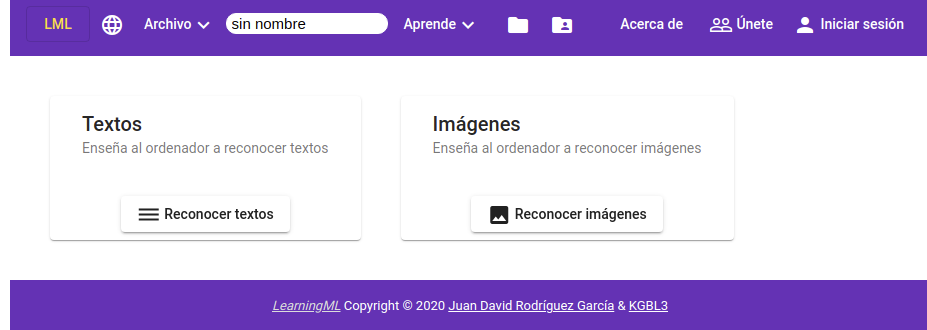
\includegraphics[width=13cm, keepaspectratio]{img/LearningML.png}
	\caption{Página de inicio de LearningML.} \label{fig:learningML}
\end{figure}

\section{Angular} 
\label{sec:Angular}

Angular~\cite{Pagina_de_angular, Curso_de_angular} es un \emph{framework} de código abierto desarrollado por Google que mediante el uso de TypeScript y HTML permite crear aplicaciones de una sola página, denominadas SPA (\emph{Single Page Application}).

Angular nació en 2010 con el nombre de AngularJS pero en el año 2016 pasó a llamarse Angular, en su versión 2.0 y ha ido evolucionando e implantando mejoras. 
La última versión es la 13 publicada en noviembre de 2021.

Las ventajas que tiene Angular es que mantiene la aplicación más ordenada, simplifica el código y evita escribir código repetitivo gracias a que sigue un modelo MVC (\emph{Modelo-Vista-Controlador}), a la vez que posibilita que las modificaciones y las actualizaciones de las aplicaciones sean rápidas y sencillas. 
Además, separa el \emph{frontend} y el \emph{backend} en la aplicación.

La principal ventaja que tienen las SPA es que tiene una alta velocidad de carga entre las vistas que tiene la aplicación web, ya que cuando hay un cambio de vista no se recarga la página, sino que las vistas se cargan de forma rápida, dinámica y reactiva. 
Esto se debe a que solamente hay una petición inicial al servidor y una respuesta HTML del mismo. Luego funciona mediante routing que es un servicio con el que se puede implementar una navegación basada en rutas, cada ruta de angular sirve para mostrar la vista de un determinado componente.

Como cualquier \emph{framework}, Angular tiene una serie de librerías que se pueden importar para facilitar el desarrollo del código, o para solucionar problemas concretos. 
Las librerías amplían las funcionalidades.

La arquitectura de una aplicación Angular está basada en cuatro clases distintas, que se identifican a través de decoradores. 
Estos decoradores definen su tipo y proporcionan metadatos que le indican a Angular cómo usarlos.
Las cuatro clases que utiliza son:

\begin{itemize}

	\item[•] \textbf{Módulos:} declaran un contexto de compilación para un conjunto de componentes. 
	Los módulos juegan un papel fundamental en la estructuración de las aplicaciones Angular. 
	Es donde se definen o declaran los componentes, las directivas y los servicios que conforman la aplicación. 
	Los módulos representan una agrupación lógica de lo que podríamos llamar áreas funcionales de una aplicación. 
	También definen las rutas que establecen las vistas de la aplicación y las dependencias con otros módulos, es decir, qué módulos necesita importar y qué componentes o directivas exporta. 
	
	Cualquier aplicación de Angular tiene un módulo raíz, llamado \texttt{AppModule}, que proporciona el mecanismo de arranque que inicia la aplicación, pero no es el único, normalmente una aplicación contiene varios módulos funcionales, además de los propios del \emph{framework}. 
	
	Los módulos de Angular pueden importar o exportar funcionalidades de otros módulos, esto hace que cada módulo sea independiente. 
	La organización en distintos módulos ayuda a gestionar el desarrollo de aplicaciones complejas y a la reutilización de código.
	
	Para definir una clase como módulo se utiliza el decorador \texttt{@NgModule}.
	
	\item[•] \textbf{Componentes:} son los bloques de construcción que componen una aplicación, contienen la lógica y los datos de la aplicación. 
	Cada componente tiene asociada una plantilla HTML. Las plantillas son las vistas que conforman la interfaz de usuario y se cargan cuando se cambia o modifica la URL.
	
	Una aplicación de Angular tiene al menos el componente raíz, llamado \texttt{AppComponent}, que conecta una jerarquía de componentes con el modelo de objeto del documento (DOM) de la página.
	
	Los componentes pueden tener uno o varios subcomponentes. Estos pueden relacionarse entre sí de dos formas: i) mediante eventos para actualizar datos cuando el usuario interacciona con la interfaz gráfica, ii) mediante las propiedades o interpolación para enviar datos a las plantillas que conforman las vistas. 
	Esto hace que los cambios en el DOM puedan modificar los datos de la aplicación y los datos de la aplicación puedan modificar las plantillas.
	
	Para definir una clase como componente se utiliza el decorador \texttt{@NgComponent}.
	
	\item[•] \textbf{Directivas:} son clases que agregan comportamiento adicional a los elementos en sus aplicaciones Angular para modificar de alguna manera el código HTML. 
	Antes de que se muestre una vista, Angular evalúa las directivas y resuelve la sintaxis vinculante en la plantilla para modificar los elementos HTML y el DOM.
	
	Hay tres tipos de directivas:
	
	\begin{enumerate}
	\item Directivas de componente: los componentes son un tipo de directiva.
	\item Directivas de atributos: modifican el comportamiento o la apariencia de un elemento, componente o directiva.
	\item Directivas estructurales: modifican la apariencia agregando y eliminando elementos del DOM.
	\end{enumerate}
	
	Se pueden crear directivas o Angular dispone de directivas integradas que se pueden usar para administrar formularios, listas, estilos y lo que ven los usuarios. 
	Algunos ejemplos de directivas de atributos integradas son \texttt{NgClass}, \texttt{NgStyle} y \texttt{NgModel}, y de directivas estructurales \texttt{NgIf}, \texttt{NgFor} y \texttt{NgSwitch}.
	
	\item[•] \textbf{Servicios:} proporcionan una funcionalidad específica que no está directamente relacionada con las vistas. Los servicios son clases con un propósito limitado y bien definido, deben hacer algo específico y de uso general. 
	Se usan para cambiar datos entre componentes, obtener datos del servidor, validar la entrada del usuario o cualquier servicio que se repita en distintas componentes.
	
	Angular distingue los componentes de los servicios para aumentar la modularidad y la reutilización. 
	Al separar la funcionalidad relacionada con la vista de un componente de otros tipos de procesamiento, puede hacer que sus clases de componentes sean sencillas y eficientes.
	
	Para definir una clase como servicio se utiliza el decorador \texttt{@Injectable}, ya que proporciona los metadatos que permiten inyectar otros proveedores como dependencias en su clase.
	
\end{itemize}


\subsection{Angular CLI}
\label{subsec:Angular CLI}

Angular CLI (\emph{Command Line Interface})~\cite{Pagina_de_angular_CLI} es una herramienta de interfaz de línea de comandos desarrollada por Angular que se utiliza para inicializar, desarrollar, montar y mantener aplicaciones de Angular directamente desde un shell de comandos. 

Es una herramienta que facilita el inicio de una aplicación de Angular, porque, con una instrucción \texttt{ngnew}, crea una carpeta de trabajo y genera el esqueleto de aplicación. 
También tiene instrucciones que permiten crear nuevas clases de forma sencilla, creando los distintos archivos que forman un módulo, componente, servicio o una directiva, además de incluirlos en los archivos necesarios y crear las dependencias. 
Las herramientas predefinidas más destacadas son el servidor web, el compilador y el sistema de testeo.

\subsection{MVC}
\label{subsec:MVC}

Para el desarrollo de una aplicación web Angular utiliza el patrón MVC (\emph{Modelo-Vista-Controlador})~\cite{Pagina_MVC} que se utiliza para separar en tres componentes los datos, la metodología y la interfaz gráfica de una aplicación, lo que permite modificar cada uno de ellos sin tener que modificar los demás. 
La arquitectura MVC está formada por tres componentes, que son:
	\begin{itemize}
	\item[•] \textbf{Modelo:} es el encargado de la manipulación, gestión y actualización de los datos. 
	En el caso de que haya una base de datos es donde se realizan las consultas, búsquedas o actualizaciones.  
	
	\item[•] \textbf{Vista:} es la representación gráfica de los datos proporcionados por el controlador. 
	Ni el controlador ni el modelo se preocupan de cómo se verán los datos, toda la parte del diseño de la interfaz es responsabilidad de la vista.
	
	\item[•] \textbf{Controlador:} es el componente principal. Se encarga de gestionar las instrucciones que se reciben del usuario, atenderlas y procesarlas. 
	Después realiza las consultas al modelo y una vez se hayan obtenido dichos datos, se envía a la vista para producir una salida como respuesta al evento.
	\end{itemize}
	
Las ventajas que aporta esta arquitectura son: facilita el mantenimiento, permite la reutilización de componentes y mejora la escalabilidad, ya que separa cada tipo de lógica.

\section{HTML5} 
\label{sec:HTML5}

HTML (\emph{HyperText Markup Language})~\cite{Pagina_HTML, Historia_HTML5, gauchat2012gran} es un lenguaje de marcado que se utiliza para definir la estructura y el contenido de una página Web, y es el componente más básico de una web. 
Se escribe en texto plano y tiene una estructura de árbol de elementos y textos. 
La estructura básica de un documento HTML se compone de los siguientes elementos: \texttt{<!DOCTYPE>}, \texttt{<html>}, \texttt{<head>} y \texttt{<body>}. 
HTML provee los elementos estructurales y se complementa con CSS (\emph{Cascading Style Sheets}) para modificar la apariencia de la página y con JavaScript para proveer dinamismo y construir aplicaciones web completamente funcionales. 

La idea de desarrollar HTML5 nació en 2004, cuando el consorcio W3C (\emph{World Wide Web Consortium}) que está a cargo del estándar decidió dejar de evolucionar HTML. Debido a esto la asociación WHATWG (\emph{Web HyperText Application Technology Working Group}), formada por Apple, Opera y Mozilla, decidió crear HTML5 y publicó el primer borrador de HTML5. 
En el año 2007 W3C formó un grupo de trabajo autorizado para trabajar con WHATWG en el desarrollo de HTML5, pero en 2011 se separaron debido a que tenían distintos objetivos: W3C quería publicar una versión terminada, mientras que WHATWG quería seguir trabajando en una constante evolución de HTML5. 
En 2019, WHATWG y W3C firmaron un acuerdo para colaborar en una única versión de HTML en el futuro.

HTML5 fue creado con la intención de hacerlo más eficiente que las versiones anteriores, mantener la compatibilidad con versiones anteriores y facilitar el desarrollo web compatible con distintos navegadores. Las principales novedades de HTML5 son:

	\begin{itemize}
	\item[•] Incorpora nuevas etiquetas que permiten una mejor estructuración de los documentos HTML, ya que antes solo estaba el \texttt{<div>} para definir secciones. 
	Ahora se pueden utilizar también \texttt{<header>} para la cabecera, \texttt{<section>} para la información principal, \texttt{<nav>} para la barra de navegación y \texttt{<footer>} para el pie, entre otros.
	\item[•] Permite incorporar elementos multimedia para reproducir audios y videos desde el propio navegador, con las etiquetas \texttt{<audio>} y \texttt{<video>}.
	\item[•] Incluye numerosas APIs, algunas de ellas son:
		\begin{itemize}
		\item Forms: incluye mejoras en los formularios para personalizar todos los aspectos de procesamiento y validación.
		\item Canvas: permite dibujar, presentar gráficos en pantalla, animar y procesar imágenes y texto.
		\item Geolocation: permite a los desarrolladores determinar la ubicación física real del usuario y e mostrar e interactuar con un mapa de Google Maps.
		\item Drag and drop: permite arrastrar un elemento desde un lugar y luego soltarlo en otro.
		\item Web Storage: es una mejora de las cookies y permite el almacenamiento local en el lado del cliente, con \texttt{localStorage}, cuando la información tiene que estar disponible solo durante la sesión y \texttt{sessionStorage}, cuando tiene que ser preservada todo el tiempo que el usuario desee.
		\end{itemize}
	\end{itemize}


\section{CSS3} 
\label{sec:CSS3}

CSS3 (\emph{Cascading Style Sheets})~\cite{gauchat2012gran} es la última versión de CSS. 
Es un lenguaje de diseño gráfico que permite definir y crear el aspecto visual de los documentos HTML. 
Es un complemento desarrollado para superar las limitaciones y reducir la complejidad de HTML, por lo que se separa el estilo del documento de la estructura y el contenido de este. 
Esta separación permite que varios documentos HTML tengan la misma hoja de estilo, simplificando el trabajo de los desarrolladores, o que un mismo documento HTML pueda tener distintos estilos, permitiendo variaciones en la visualización para diferentes dispositivos y tamaños de pantalla.

El consorcio W3C es el encargado de definir y mantener las especificaciones de este lenguaje. 
Las principales novedades de CSS3 son: esquinas redondeadas, sombras en cajas y textos, elegir la fuente del texto, gradientes, opacidad y transparencia de los colores, incluir transiciones, entre otras.

\section{TypeScript} 
\label{sec:TypeScript}

TypeScript~\cite{Pagina_de_typescript} es un lenguaje de programación de código abierto desarrollado y mantenido por Microsoft. 
Es un superconjunto de JavaScript, es decir, amplía JavaScript con una nueva sintaxis que añade tipos estáticos y objetos basados en clases. 
Nació en 2012 como solución para el desarrollo de aplicaciones  robustas y de gran tamaño, ya que con JavaScript era muy complicado debido a su escasa escalabilidad. 
Su uso está permitido tanto en el lado del cliente como en el lado del servidor con Node.js

 Los programas de JavaScript son compatibles en TypeScript, por lo que se puede integrar en proyectos ya existentes porque a través de un compilador de TypeScript se traducen a código JavaScript. 
Además, tiene las herramientas de JavaScript ES6 y JavaScript ES7. De esta manera se mantiene actualizado con las últimas mejoras de JavaScript. 
Los cambios más importantes respecto a JavaScript son:

\begin{itemize}
	\item[•] Evita errores en tiempo de ejecución, ya que incorpora tipado estático, es decir, al crear variables se puede añadir el tipo de dato.
	
	\item[•] Es más funcional porque al añadir objetos basados en clases hace que la programación orientada a objetos sea más sencilla.
\end{itemize}

En la actualidad se encuentra en la versión 2.0 que introduce varias características, entre ellas la capacidad de evitar la asignación de variables con un valor nulo. 

\section{Node.js} 
\label{sec:Node}

Node.js~\cite{Pagina_de_Node} fue creado por Ryan Dahl en 2009. Es un entorno en tiempo de ejecución de JavaScript orientado a eventos asíncronos, diseñado para construir aplicaciones de red escalables, como por ejemplo, servidores web. 
Está influenciado por sistemas como Event Machine de Ruby y Twisted de Python.

Con Node.js el código JavaScript, no se ejecuta en un navegador, sino en el servidor. Utiliza el motor V8 de Google para interpretar y ejecutar el código JavaScript, suministrando un entorno de ejecución en el lado del servidor, del mismo modo que hace el navegador cuando se utiliza JavaScript en el lado del cliente.

Al estar orientado a eventos asíncronos puede soportar una gran cantidad de conexiones. 
Esto lo diferencia del modelo de concurrencia más común, en el que se emplean hilos del Sistema Operativo. En estos SC se usa un hilo por cada conexión, lo que provoca que si se tienen muchas conexiones es necesaria mucha capacidad de memoria. 
Node.js utiliza un único hilo de ejecución y un bucle de eventos asíncrono, tratando las nuevas conexiones como un nuevo evento dentro del bucle. Cada conexión recibe una pequeña asignación de espacio de memoria dinámico, sin tener que crear un hilo de ejecución, evitando que se produzcan bloqueos en el flujo de trabajo. 

\section{TensorFlow} 
\label{sec:TensorFlow}

TensorFlow~\cite{Pagina_de_TensorFlow} es el sistema de aprendizaje automático de segunda generación de Google Brain, liberado como software de código abierto en 2015, por lo que el acceso a esta herramienta es libre y es posible editarla en función de las necesidades. 

Es una plataforma para construir y entrenar redes neuronales para detectar y descifrar patrones y correlaciones, parecidos al aprendizaje y razonamiento usados por los humanos. 
Tiene un ecosistema integral y flexible de herramientas, bibliotecas y recursos de la comunidad que permite a los desarrolladores crear e implementar fácilmente aplicaciones basadas en ML.


\section{JSON} 
\label{sec:JSON}

JSON (\emph{JavaScript Object Notation})~\cite{Pagina_de_JSON} es un formato ligero de intercambio de datos. Es fácil de leer y escribir para los humanos, mientras que para las máquinas es sencillo de interpretar y generar. 
A pesar de que está basado en un subconjunto del lenguaje de programación JavaScript, es un formato de texto completamente independiente del lenguaje. JSON está construido por dos estructuras:

\begin{enumerate}
	\item Objeto: colección de pares de nombre/valor. Comienza con una llave de apertura y termina con una llave de cierre, cada nombre es seguido de dos puntos y los pares nombre/valor están separados por una coma.
	\item Array: lista ordenada de valores. Comienza con un corchete izquierdo y termina con un corchete derecho, los valores se separan por comas.
\end{enumerate}

Estas estructuras pueden anidarse y los valores pueden ser:
	\begin{itemize}
		\item[•] Cadena de caracteres. Se ponen entre comillas dobles.
		\item[•] Números. Pueden contener parte fraccional separada por un punto y se permiten números negativos.
		\item[•] Booleanos. True y false.
		\item[•] Null. Representa el valor nulo.
	\end{itemize}

\section{Conjunto de datos} 
\label{sec:dataset}

Un conjunto de datos o dataset es una colección de datos tabulados, es decir, en forma de tabla. 
Las columnas de la tabla son los atributos, que son el nombre de las características de los datos. 
Las filas de la tabla son las muestras con los datos de los atributos. Los datos pueden ser numéricos y categóricos, es decir, cadenas de caracteres. 
Las muestras se agrupan en clases. Una clase tiene muestras con valores similares por lo que las muestras definen como es una clase. 
Un ejemplo de un conjunto de datos muy utilizado en el aprendizaje automático es el \emph{conjunto de datos flor iris}\footnote{\url{https://es.wikipedia.org/wiki/Conjunto_de_datos_flor_iris}}, que está compuesto por tres clases que son tres especies de la flor iris (iris setosa, iris virginica e iris versicolor), cuatro atributos (largo de sépalo, ancho de sépalo, largo de pétalo y ancho de pétalo) y 50 muestras de cada clase que definen cómo es cada flor.

%%%%%%%%%%%%%%%%%%%%%%%%%%%%%%%%%%%%%%%%%%%%%%%%%%%%%%%%%%%%%%%%%%%%%%%%%%%%%%%%
%%%%%%%%%%%%%%%%%%%%%%%%%%%%%%%%%%%%%%%%%%%%%%%%%%%%%%%%%%%%%%%%%%%%%%%%%%%%%%%%
% DISEÑO E IMPLEMENTACIÓN %
%%%%%%%%%%%%%%%%%%%%%%%%%%%%%%%%%%%%%%%%%%%%%%%%%%%%%%%%%%%%%%%%%%%%%%%%%%%%%%%%

\cleardoublepage
\chapter{Diseño e implementación} 

\section{Arquitectura de LearningML} 
\label{sec:arquitectura}

La arquitectura de \texttt{LearningML} está construida con Angular, por lo que está compuesta por módulos, componentes y servicios, de manera que es sencillo realizar cambios o añadir funcionalidades. 

En la figura~\ref{fig:arquitectura} se puede ver la arquitectura general de \texttt{LearningML}. El servicio \texttt{labeled-data-
manager} es de uso general y lo importan la mayoría de componentes y algunos sevicios, ya que se encarga de guardar los datos que necesitan los servicios y componentes. 
Luego está el componente \texttt{ml-home} que se corresponde con la página principal y es donde se selecciona qué tipo de reconocimiento se desea realizar, de textos o de imágenes. Una vez se ha seleccionado, se pasa al componente \texttt{ml-model} mediante routing con el módulo \texttt{app-routing} que funciona mediante rutas, por lo que además de cambiar de componente también se cambia de página. 
En función del reconocimiento escogido se mostrarán unos elementos u otros del HTML de \texttt{ml-model}.

En el componente \texttt{ml-model} se importan los servicios \texttt{feature-extraction} y \texttt{ml-algorithm}. A su vez el primero importa dos servicios: \texttt{feature-extractor-text} y \texttt{feature-extractor-
image}, y el segundo importa otros dos servicios: \texttt{ml-algorithm-knn} y \texttt{ml-algorithm-
neural-networks}.

El componente \texttt{ml-model} es el constructor del modelo y está dividido en tres secciones. La primera es donde se introducen los datos de entrenamiento; primero se introducen las distintas clases a las que puede pertenecer una entrada y una vez se ha introducido al menos una clase, entra en funcionamiento el componente \texttt{ml-label-container} que es donde se recogen las entradas de cada clase con los datos que se utilizan en la segunda sección, la parte de aprendizaje. \\
En la parte de aprendizaje es donde se utiliza la función \texttt{train} que es donde realmente se realiza la construcción del modelo y se entrena. Primero se realiza la extracción de características mediante el servicio \texttt{feature-extraction} y este es el que elige, dependiendo del tipo de dato, cuál de los dos servicios usar para la extracción de características. 
Después llama a \texttt{ml-algorithm}, y este servicio decide que algoritmo utilizar para construir y entrenar el modelo para el reconocimiento. 
Por defecto utiliza el algoritmo \texttt{ml-algorithm-neural-networks}, pero se puede seleccionar el modo avanzado en el cual se puede elegir entre los dos y modificar los parámetros del algoritmo.\\
Cuando el modelo ya está entrenado se pasa a la tercera sección, la parte de evaluación. Aquí es donde se realizan las pruebas de reconocimiento. 
En función del reconocimiento escogido se hace uso del componente \texttt{ml-test-text-model} o del componente \texttt{ml-test-image-model}. 
Primero llaman a \texttt{feature-extraction} y después a \texttt{ml-algorithm}, igual que \texttt{ml-model}.

\begin{figure}
	\centering
	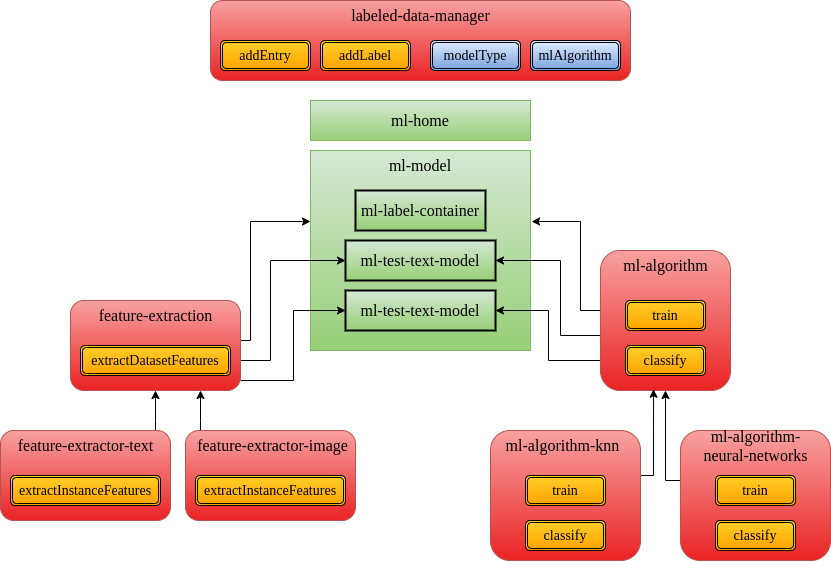
\includegraphics[width=13cm, keepaspectratio]{img/arquitectura.png}
	\caption{Arquitectura general de \texttt{LearningML}. En rojo los servicios, en verde los componentes, en amarillo las funciones y en azul las variables.} \label{fig:arquitectura}
\end{figure}

En la figura~\ref{fig:arquitectura} también se puede observar qué contiene principalmente cada servicio nombrado anteriormente. Estos servicios tienen un desempeño específico:

\begin{itemize}
	\item[•] labeled-data-manager: es el encargado de guardar datos, que son características que definen el modelo. \texttt{labeled-data-manager} guarda las etiquetas, es decir, las clases a las que puede pertenecer una entrada. Esto se hace con la función \texttt{addLabel}, que guarda las etiquetas en un array en la variable \texttt{labels} y en un objeto Map en la variable \texttt{labelsWithData}. 
	\texttt{labeled-data-manager} guarda los datos de entrada, ya sean textos o imágenes, con la función \texttt{addEntry} que los guarda en la variable \texttt{labelsWithData} junto con la clase en la que ha sido añadida la entrada para así tener cada etiqueta con sus datos, y guarda el tipo de modelo que se va a construir, es decir, el tipo de reconocimiento seleccionado, en la variable \texttt{modelType}. También se encarga de guardar el tipo de algoritmo en la variable \texttt{mlAlgorithm}. \\
	Además de guardar estos datos también borra etiquetas o entradas y se encarga de guardar o cargar los datos de un JSON tanto del ordenador como de la nube si el usuario está registrado.
	
	\item[•] feature-extraction: es el encargado de llamar a los otros dos servicios en función de si se quieren extraer características de un texto o de una imagen mediante la función \texttt{extractDatasetFeatures}. Los servicios son:
	
	\begin{itemize}
		\item feature-extractor-text: es el encargado de extraer las características de los textos, es decir, convertir un texto en un tensor. 
		La función que lo convierte en un tensor es \texttt{extractInstanceFeatures}
		
		\item feature-extractor-image: es el encargado de extraer las características de las imágenes, es decir, convertir una imagen en un tensor. 
		La función que lo convierte en un tensor es \texttt{extractInstanceFeatures} al igual que en el caso de los textos.
	\end{itemize}
	
	\item[•] ml-algorithm: es el encargado de llamar a los otros dos servicios en función del algoritmo que se utilice. 
	Tiene dos funciones principales, \texttt{train} y \texttt{classify}, con las que llama a los otros servicios para entrenar o clasificar. Los servicios son:
	
	\begin{itemize}
		\item[*] ml-algorithm-knn: se usa en caso de que el algoritmo elegido sea K-KNN. 
		Tiene dos funciones que son las que llama el servicio \texttt{ml-algorithm}, \texttt{train} para entrenar o \texttt{classify} para clasificar.
		\item[*] ml-algorithm-neural-networks: tiene las mismas funciones que K-KNN, pero en este caso entrena o evalúa utilizando el algoritmo de redes neuronales.
	\end{itemize}
\end{itemize}

\section{Cambios en la arquitectura de LearningML} 
\label{sec:arquitectura nueva}

Realizar cambios en la arquitectura no fue complicado, ya que la aplicación está hecha para poder realizar cambios e implementar nuevas funcionalidades. 
Solo hay que entender cómo está estructurada y qué es lo que hace cada parte.

Para añadir la nueva funcionalidad tenía dos opciones en cuanto a la construcción del modelo: crear un nuevo componente o añadir la funcionalidad en el componente \texttt{ml-model}. Nos decidimos por la segunda para seguir con la misma estructura, ya que no había un componente diferente para construir el modelo de textos y otro para imágenes, por lo que nos parecía más lógico seguir con la misma dinámica.

\begin{figure}[b!]
	\centering 
	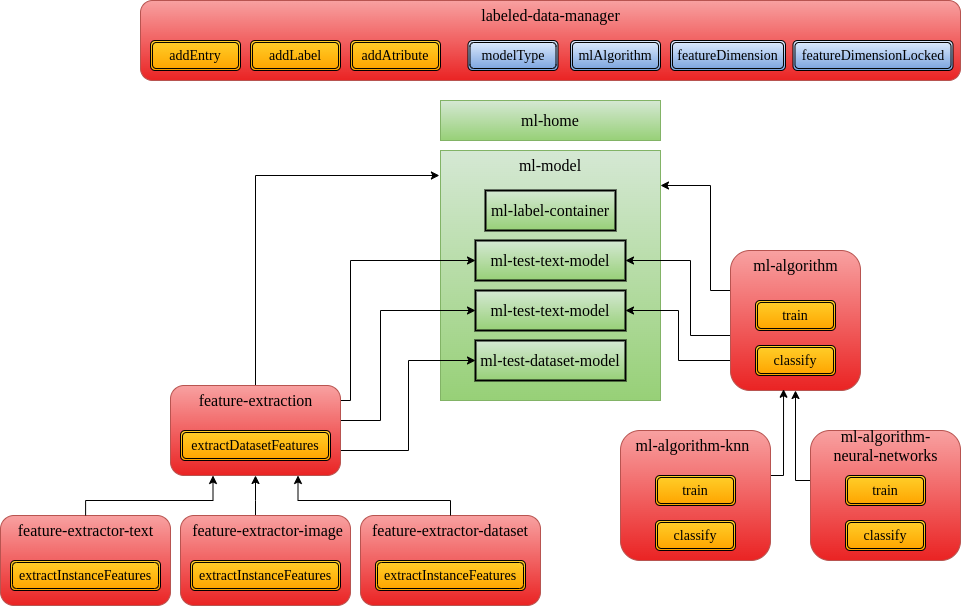
\includegraphics[width=13cm, keepaspectratio]{img/arquitectura_nueva.png}
	\caption{Arquitectura nueva de \texttt{LearningML}. En rojo los servicios, en verde los componentes, en amarillo las funciones y en azul las variables.} \label{fig:arquitectura_nueva}
\end{figure}

Los cambios en la arquitectura se pueden observar en la figura~\ref{fig:arquitectura_nueva}. 
Se ha añadido el componente \texttt{ml-test-dataset-model} para realizar la evaluación cuando el tipo de reconocimiento es de conjuntos de datos. Este tiene la misma funcionalidad que cuando son textos o imágenes, pero adaptado al tipo de datos que tiene un conjunto de datos y sigue utilizando e importando los servicios \texttt{feature-extraction} y \texttt{ml-algorithm}. Para indicar cómo son ese tipo de datos se añadieron en el fichero \texttt{interfaces}. \\
También se ha añadido el servicio \texttt{feature-extractor-dataset} para extraer las características de los conjuntos de datos, es decir, convertir un conjunto de datos en un tensor. 
La función que lo convierte en un tensor es \texttt{extractInstanceFeatures} al igual que en el caso de textos e imágenes.

Además, en el servicio \texttt{labeled-data-manager} se ha añadido la función \texttt{addAtribute} para guardar los atributos del conjunto de datos en un array en la variable \texttt{attributes}. 
Se han añadido variables para manejar cambios que se producen en el modelo como son \texttt{addAttributeLocked} y \texttt{featureDimensionLocked}. Estas son variables booleanas que cambian de valor cuando se cumple una condición; la condición son cambios en el modelo. 
También se ha añadido la variable \texttt{featureDimension} en la que se guarda el número de atributos que va a tener el modelo. \\
Como este servicio también se encarga de cargar los datos de un JSON, se ha añadido el caso en las funciones \texttt{load} y \texttt{loadFromServer} para cuando el \texttt{modelType} es \emph{dataset}. 
Para cuando se guardan los datos, se ha creado un nuevo objeto para cuando se genere el JSON, ya que ahora además de tener \texttt{type} con el tipo de modelo y \texttt{data} con las clases y sus entradas, también tiene \texttt{attributes} con los atributos. 
Para esto se ha creado la función \texttt{getDataObject} que es llamada por la función \texttt{serializeModel}, que a su vez es llamada por las funciones \texttt{save} y \texttt{saveOnServer}.


\section{Cambios en la interfaz de LearningML} 
\label{sec:interfaz}

Los cambios realizados en la interfaz de usuario son:

\begin{itemize}
	\item[•] En el componente \texttt{ml-home} se ha añadido un container para el conjunto de datos como se puede ver en la figura~\ref{fig:pagina_principal}.
	\item[•] En el componente \texttt{ml-model} se han realizado cambios en dos de las tres secciones:
	\begin{itemize}
		\item Sección de entrenamiento: hay que crear el conjunto de datos, por lo que se añade un \emph{div} para cuando el \texttt{modelType} es \emph{dataset}, porque ya no se introducen las clases lo primero. 
		Ahora hay que indicar el número de atributos que tiene el dataset, mediante un input. 
		A continuación hay que añadir los atributos, mediante un botón. 
		Si el número de atributos es correcto se muestran debajo en un desplegable. 
		Una vez se tiene definido como va a ser el dataset, es decir, se tienen añadidos los atributos, aparece el botón para añadir una clase a la que puede pertenecer una entrada. Esta parte está igual que antes. 
		En la figura~\ref{fig:entrenar} se puede observar cómo queda la sección de entrenamiento una vez introducidos los atributos.\\
		También se añade una ventana emergente para cuando hay que añadir los atributos, ya que es diferente a cuando hay que añadir una clase. El fichero se llama \texttt{ml-add-attribute-dialog}.

\begin{figure}
	\centering 
	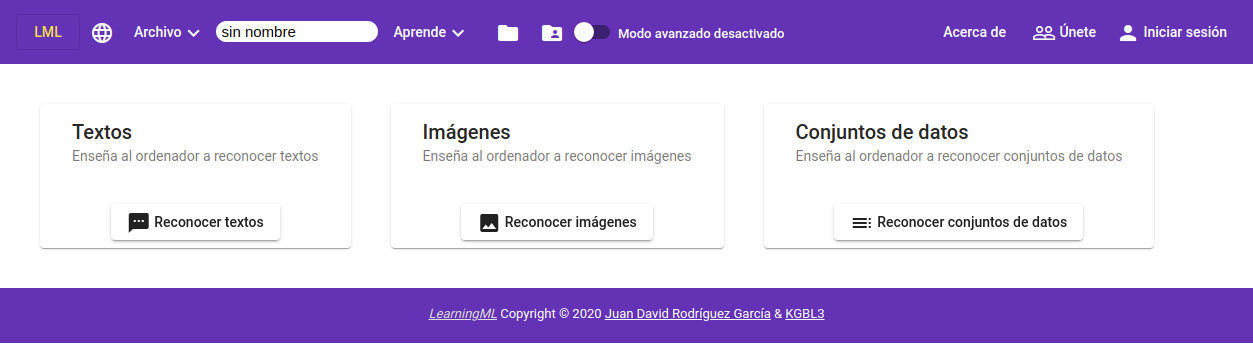
\includegraphics[width=13cm, keepaspectratio]{img/pag_principal.png}
	\caption{Página principal de \texttt{LearningML}.} \label{fig:pagina_principal}
\end{figure}

\begin{figure}
	\centering 
	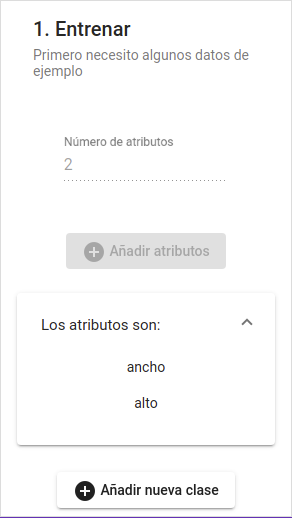
\includegraphics[width=5cm, keepaspectratio]{img/entrenar.png}
	\caption{Sección de entrenamiento de \texttt{ml-model}.} \label{fig:entrenar}
\end{figure}

\begin{figure}
	\centering
	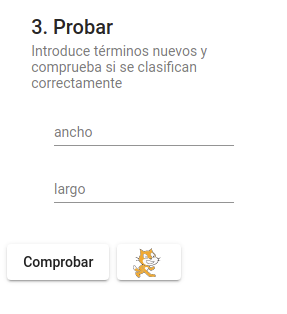
\includegraphics[width=5cm, keepaspectratio]{img/probar.png}
	\caption{Componente \texttt{ml-test-dataset-model}.} 	\label{fig:probar}
\end{figure}

		\item Sección de evaluación: se ha añadido la etiqueta con el selector del componente \\ \texttt{ml-test-dataset-model}.
	\end{itemize}
	
	\item[•] En el componente \texttt{ml-test-dataset-model} se muestran tantos inputs como número de atributos se hayan indicado y cada uno corresponde con un atributo para introducir los valores de cada atributo y comprobar si se clasifican correctamente. 
	Se puede observar en la figura~\ref{fig:probar}.
\end{itemize}


\section{Creación de conjuntos de datos} 
\label{sec:crear conjunto de datos}

Los conjuntos de datos se pueden crear o se pueden importar en formato JSON. En esta sección se explica cómo crearlo desde \texttt{LearningML}. 
Se crea en el componente \texttt{ml-model} en la sección de entrenamiento y en el componente \texttt{ml-label-container}. 
Al ser una colección de datos tabulados el conjunto se divide: en atributos, en ejemplares o muestras y en clases. 

\subsection{Atributos}
\label{subsec:atributos}

Los atributos son lo primero que se le solicita al usuario, ya que define cómo va a ser el dataset. 
Este proceso se realiza en el componente \texttt{ml-model}. 
Primero hay que indicar el número de atributos que tiene el dataset y se guarda en la variable \texttt{featureDimension} de \texttt{labeled-data-manager}. Por defecto tiene dos atributos. 
Después, al pulsar el botón para añadir los atributos, éste llama a la función \texttt{addAttribute} que deshabilita el input de introducción de número de atributos. Esto es posible gracias a la variable \texttt{featureDimensionLocked} de \texttt{labeled-data-manager}.
A continuación, abre la ventana emergente \texttt{ml-add-attribute-
dialog} para escribir los atributos separados por comas. 
Si el número de atributos introducidos coincide con los de la variable \texttt{featureDimension} y todos tienen asignado un valor, es decir, se ha escrito antes y después de cada coma, se mandan los atributos a la función \texttt{addAttribute} de \texttt{labeled-data-manager} para guardarlos y poder mostrarlos debajo en un desplegable para tener presente cuales son las características que tienen que tener los datos de entrada y para bloquear el botón para añadir atributos gracias a la variable \texttt{addAttributeLocked}. 
En el caso de no introducir los atributos correctamente, éstos no se guardan y sigue activo el botón para añadir atributos hasta que se introduzcan correctamente.

El input para indicar el número de atributos y el botón para añadir atributos se bloquean porque todo el dataset tiene que tener la misma forma, es decir, todas las entradas deben de tener el mismo número de atributos. Si se han añadido entradas y luego se modifica el número de atributos las entradas no van a coincidir en el número de atributos y esto no puede pasar.

\subsection{Clases}
\label{subsec:clases}

Una vez se han añadido los atributos, se pueden añadir las clases del conjunto de datos, en este caso el botón no se bloquea en ningún momento, por lo que no es necesario crear todas las clases del conjunto de datos antes de introducir las entradas de cada clase, sino que en cualquier momento se puede añadir una clase. 

Para añadir clases no se ha añadido nada, funciona como antes. 
El botón para añadir una nueva clase llama a la función \texttt{addLabel} que abre una ventana emergente para escribir la clase y luego manda el valor introducido a la función \texttt{addLabel} de \texttt{labeled-data-manager} para guardarlo en las variables \texttt{labels} y \texttt{labelsWithData}. 
La variable \texttt{labelsWithData} está compuesta de pares de datos clave-valor \{\texttt{label}, \texttt{data}\}. Cuando se añade una clase se añade un par de datos clave-valor, por lo que hay tantos pares de datos como clases tenga el conjunto de datos.

\subsection{Muestras}
\label{subsec:datos}

Las muestras de cada clase se añaden en el componente \texttt{ml-label-container}. Para ello, se ha creado la función \texttt{addRowToDataset} porque la forma que tienen las entradas es diferente: añade una fila con los valores de los atributos en la clase que se quiere añadir. 

Primero abre una ventana emergente para añadir los valores separados por comas. Si el número de valores introducidos coincide con el número de atributos de la variable \texttt{featureDimension} de \texttt{labeled-data-manager}, todos tienen asignado un valor (se ha escrito antes y después de cada coma) y la muestra no está repetida (no contiene los mismos valores y en el mismo orden que otra ya introducida en esa clase). Entonces escribe la muestra en la interfaz de usuario y manda la muestra a la función \texttt{addEntry} de \texttt{labeled-data-manager} que guarda la muestra en la variable \texttt{labelsWithData} en la clase que ha sido añadida. Como \texttt{labelsWithData} está compuesta de pares de datos clave-valor \{\texttt{label}, \texttt{data}\} busca la clase en la que se quiere añadir la muestra y añade el string de datos de la muestra en el array \texttt{data}. 
En la figura~\ref{fig:ejemplo1} se puede observar el aspecto que tiene \texttt{labelsWithData}. El ejemplo consta de dos pares de datos clave-valor, uno por cada clase y las muestras que pertenecen a cada clase.

\begin{figure}
	\centering
	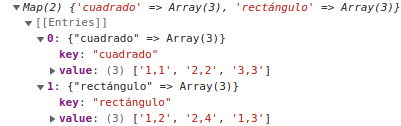
\includegraphics[width=9cm, keepaspectratio]{img/ejemplo1.png}
	\caption{Aspecto de \texttt{labelsWithData}.} 	\label{fig:ejemplo1}
\end{figure}


\section{Extracción de características}
\label{subsec:caracteristicas}

Una vez se tiene el conjunto de datos creado, se procede al entrenamiento del modelo. Para ello hay que hacer la extracción de características, es decir, convertir las muestras de las diferentes clases guardadas en la variable \texttt{labelsWithData} en tensores. En la figura~\ref{fig:extraccion_caract} se puede observar un diagrama de como se realiza la extracción de características de forma visual, se explica más detalladamente a continuación.

\begin{figure}
	\centering
	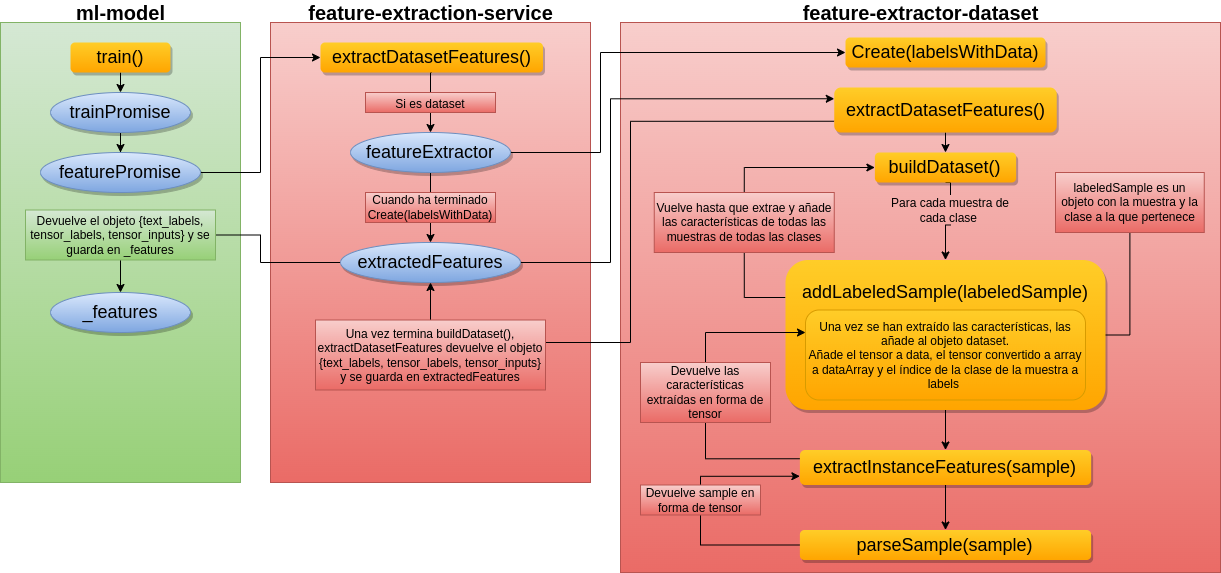
\includegraphics[width=17cm, keepaspectratio]{img/extraccion_de_caracteristicas.png}
	\caption{Diagrama de extracción de características. En verde componente, en rojo servicios, en amarillo funciones y en azul variables} 	\label{fig:extraccion_caract}
\end{figure}

Cuando se pulsa el botón aprender, éste llama a la función \texttt{train} de \texttt{ml-model} que crea la variable \texttt{featurePromise} en la cual se llama a la función \texttt{extractDatasetFeatures} del servicio \texttt{featureExtraction} de forma asíncrona. 
Al tratarse de programación asíncrona, se utiliza la función \texttt{then} cuya función consiste en esperar a que la función asíncrona devuelva un valor para después hacer uso de ese valor. 
En la función \texttt{extractDatasetFeatures} se crea el \texttt{feature-extractor-dataset} porque el \texttt{modelType} es \emph{dataset} y lo guarda en la variable \texttt{featureExtractor}, se crea llamando a la función \texttt{create} de \texttt{feature-
extractor-dataset} a la cual se le pasa como parámetro la variable \texttt{labelsWithData} para que el servicio \texttt{feature-extractor-dataset} guarde los datos de \texttt{labelsWithData}. 
Después llama a \texttt{extractDatasetFeatures} de \texttt{featureExtractor}.

A continuación la función \texttt{extractDatasetFeatures} de \texttt{feature-extractor-dataset} llama a la función \texttt{buildDataset} de forma asíncrona. Esta función construye el objeto \texttt{dataset} con los datos con los que pueden trabajar los algoritmos y que tiene la siguiente estructura:
\begin{verbatim}
dataset = {
    data: [],
    labels: [],
    dataArray: []
};
\end{verbatim}

\texttt{labels} es un array que contiene el índice que le corresponde a la clase de cada muestra, \texttt{data} es un array que contiene los valores de cada muestra en forma de tensor y \texttt{dataArray} es un array que contiene los valores de cada muestra en forma de array con valores numéricos.

La construcción del objeto \texttt{dataset} se hace mediante dos bucles: el primero itera sobre las clases y el segundo sobre las muestras de cada clase. 
Para cada muestra llama a la función \texttt{addLabeledSample} que recibe como parámetro un objeto con la muestra y la clase a la que pertenece la muestra. Esta función se encarga de añadir las características extraídas de cada muestra al objeto \texttt{dataset}. 
Primero comprueba si la clase está dentro de las clases conocidas por el modelo y, si no está, la añade. 
Después llama a la función \texttt{extractInstanceFeatures} de forma asíncrona y que recibe como parámetro la muestra para extraer las características, pero para ello tiene que llamar a la función \texttt{parseSamle} porque los datos de la muestra pueden ser números o una cadena de caracteres. 
La función \texttt{parseSamle} recibe como parámetro la muestra que se separa por comas y cada valor de la muestra se pasa a \emph{float}. Si \emph{float} es un número se guarda en la variable \texttt{sampleNum}, y si no es un número se comprueba si el valor de la muestra está en la variable \texttt{sampleString} que es un objeto Map clave-valor siendo la clave el valor de la muestra y el valor un id. 
Si el valor de la muestra no está en la variable \texttt{sampleString} se guarda en esa variable el valor de la muestra y en el id un número empezando por cero y sumando uno cada vez que se añada una muestra a la variable. 
Después se guarda el id de la cadena de caracteres en la variable \texttt{sampleNum}. De esta forma se asigna un número a cada cadena de caracteres y cuando se repite una cadena de caracteres tiene el mismo número asignado que se le asignó a esa cadena de caracteres la primera vez que se guardó en la variable \texttt{sampleString}. 
En la figura~\ref{fig:ejemplo2} se puede ver un ejemplo de una muestra con números y cadenas de caracteres. La muestra es 'rojo,2,azul,3' y se observa como asigna un número a una cadena de caracteres, en este caso asigna el 0 a 'rojo'y 1 a 'azul' y en la variable \texttt{sampleNum} se guarda como [0,2,1,3]. 
Cuando ya están guardados todos los valores de la muestra en la variable \texttt{sampleNum} devuelve un tensor de una dimensión a la función \texttt{extractInstanceFeatures} que a su vez devuelve las características extraídas en forma de tensor de una dimensión a la función \texttt{addLabeledSample} que añade el tensor a \texttt{data} de \texttt{dataset}, el tensor convertido a array a \texttt{dataArray} de \texttt{dataset} y el índice que le corresponde a la clase de la muestra a \texttt{labels} de \texttt{dataset}.

\begin{figure}
	\centering
	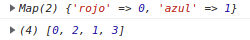
\includegraphics[width=7cm, keepaspectratio]{img/ejemplo2.png}
	\caption{Muestra con números y cadena de caracteres} 	\label{fig:ejemplo2}
\end{figure}

Cuando ya se han añadido todas las muestras de todas las clases al objeto \texttt{dataset}, la función \texttt{extractDatasetFeatures} devuelve un objeto con la siguiente estructura \{\texttt{text\_labels}, \texttt{tensor\_lables}, \texttt{tensor\_inputs}\} a la función \texttt{extractDatasetFeatures} de \\ \texttt{featureExtraction} que lo guarda en la variable \texttt{extractedFeatures} y se lo devuelve a la función \texttt{train} de \texttt{ml-model} que lo guarda en la variable \texttt{features} para pasárselo como parámetro a la función \texttt{train} de los algoritmos y entrenen con los datos del objeto.

Cuando hay que extraer las características de los datos en la parte de evaluación, el componente \texttt{ml-test-dataset-model} llama a la función \texttt{extractInstanceFeatures} de \texttt{feature-extraction} de forma asíncrona, que recibe como parámetro la muestra introducida en la parte de evaluación. 
Después esta función llama a \texttt{extractInstanceFeatures} de \texttt{feature-extractor-dataset} que le pasa como parámetro la muestra y llama a \texttt{parseSample} (igual que en la parte de entrenamiento) y luego devuelve la muestra en forma de tensor de una dimensión a la función \texttt{extractInstanceFeatures} de \texttt{feature-extraction}, que a su vez devuelve el resultado a \texttt{ml-test-dataset-model} que lo guarda en la variable \texttt{inputTensor} para pasárselo como parámetro a la función \texttt{classify} de los algoritmos y clasifiquen la muestra de forma asíncrona. 
Cuando ya ha clasificado la muestra se guarda la predicción en la variable \texttt{prediction}, que es un array que contiene tantos arrays como clases tenga el modelo, y cada array contiene el nombre de la clase y la probabilidad de que esa muestra pertenezca a esa clase, el primer array es el de mayor probabilidad y es el que se coge para escribir que es esa la clase a la que pertenece la muestra. 
También se muestra debajo los porcentajes que tiene cada clase de que la muestra le pertenezca.


%%%%%%%%%%%%%%%%%%%%%%%%%%%%%%%%%%%%%%%%%%%%%%%%%%%%%%%%%%%%%%%%%%%%%%%%%%%%%%%%
%%%%%%%%%%%%%%%%%%%%%%%%%%%%%%%%%%%%%%%%%%%%%%%%%%%%%%%%%%%%%%%%%%%%%%%%%%%%%%%%
% EXPERIMENTOS Y VALIDACIÓN %
%%%%%%%%%%%%%%%%%%%%%%%%%%%%%%%%%%%%%%%%%%%%%%%%%%%%%%%%%%%%%%%%%%%%%%%%%%%%%%%%

\cleardoublepage
\chapter{Experimentos, validación y resultados}

En esta sección se realizan algunas comprobaciones para ver si los conjuntos de datos se clasifican correctamente.
Para ello se usan dos conjuntos de datos: uno con datos numéricos y otro con datos numéricos y datos categóricos para comprobar si se guardan bien los conjuntos de datos y se extraen correctamente las características. 
Cabe destacar que todas las clases deben tener un número de muestras similar y que, cuanto mayor sea el conjunto de datos, mejor serán los resultados.

\section{Conjunto de datos numéricos}
\label{subsec:numericos}

Para comprobar la clasificación de un conjunto de datos numéricos, hemos utilizado el conjunto de datos de flor iris que se encuentra en el archivo \texttt{iris.json} de la carpeta datasets. Este dataset está compuesto de tres clases (iris setosa, iris virginica e iris versicolor) y en cada clase se han añadido 48, 49 y 50 muestras respectivamente. 
Los atributos de las muestras son longitud de sépalo, ancho de sépalo, longitud de pétalo y ancho de pétalo que son las características que diferencian una flor de otra. 
En la figura~\ref{fig:flores-iris} se pueden observar las tres flores iris y en la figura~\ref{fig:ejemplo3} se pueden observar las muestras de las distintas clases.

La creación del modelo se hace por defecto con el algoritmo de redes neuronales, pero para hacer las comprobaciones es mejor hacerlo con el modo avanzado activo. De esta forma podemos probar la validez con el algoritmo de redes neuronales y con el algoritmo de KNN.

\begin{figure}[!tb]
  \begin{center}
    \subfigure[Iris setosa.]{
        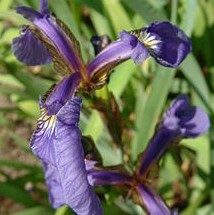
\includegraphics[width=3.25cm, keepaspectratio]{img/Iris_setosa.jpg}
        \label{flor_iris_setosa}}
    \subfigure[Iris virginica.]{
        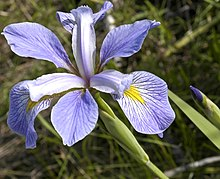
\includegraphics[width=4cm, keepaspectratio]{img/Iris_virginica.jpg}
        \label{flor_iris_virginica}}
    \subfigure[Iris versicolor.]{
        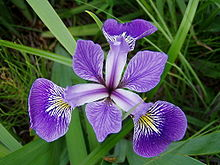
\includegraphics[width=4.3cm, keepaspectratio]{img/Iris_versicolor.jpg}
        \label{flor_iris_versicolor}}
    \caption{Tipos de flores iris.}
    \label{fig:flores-iris}
  \end{center}
\end{figure}


\begin{figure}
	\centering
	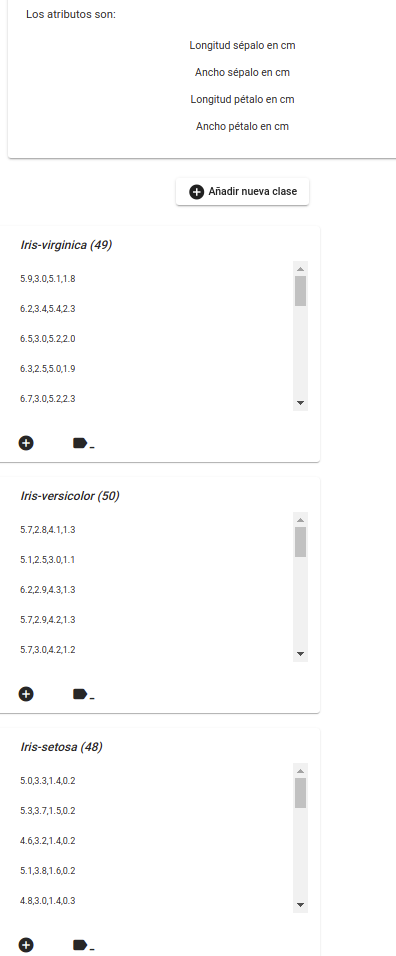
\includegraphics[width=9cm, keepaspectratio]{img/ejemplo_muestras_num.png}
	\caption{Muestras con datos numéricos para el entrenamiento} 	\label{fig:ejemplo3}
\end{figure}

\subsection{Redes neuronales}
\label{subsec:redesneuronales}

Para utilizar redes neuronales se elige el clasificador de redes neuronales en el desplegable, se seleccionan los parámetros (en este caso lo dejamos como viene), y se escoge el porcentaje de muestras que se usan como ejemplos de validación (en este caso seleccionamos un 25\%). La configuración resultante se puede observar en la figura~\ref{fig:ejemplo4}.

Hay dos formas de comprobar la validez del modelo con el algoritmo de redes neuronales:

\begin{enumerate}
 \item Con la gráfica de evolución de aprendizaje que muestra la evolución del modelo en cuanto a acierto y error a lo largo de las épocas, que son la cantidad de pases que el algoritmo de aprendizaje automático ha realizado en todo el conjunto de datos de entrenamiento. En la figura~\ref{fig:ejemplo5} se puede ver que cuantas más épocas transcurren, más aciertos hay. Al final de la gráfica, el acierto es casi 1. Esto sucede porque este algoritmo aprende de sí mismo.
Por eso según van aumentando las épocas también aumenta el porcentaje de acierto y, por consiguiente, baja el porcentaje de fallo. Este resultado indica que el aprendizaje se está realizando correctamente.
 \item Con la matriz de confusión que nos indica, en forma de tabla, los datos que predice y los que son en realidad, es decir, el número de aciertos y de fallos que ha tenido, pero no de todas las muestras sino del 25\% que se han usado como ejemplo de validación. 
En la figura~\ref{fig:ejemplo6} se puede ver un ejemplo de la matriz de confusión que en este caso tiene un 100\% de acierto, ya que de nueve muestras que predice que son de iris setosa las nueve lo son en realidad, de dieciséis muestras que predice que son iris versicolor las dieciséis son en realidad y de once muestras que predice que son iris virginica las once lo son en realidad.
Pero no siempre sale el 100\%, ya que depende de las muestras que escoja de ejemplo de validación. Habiendo comprobado bastantes veces, el fallo es muy bajo y el acierto suele ser superior al 90\% por lo que se puede considerar un porcentaje de acierto apto para realizar un buen reconocimiento de conjuntos de datos, ya que tener un acierto del 100\% es muy difícil.
 \end{enumerate} 

Con los datos obtenidos en la gráfica de evolución de aprendizaje, figura~\ref{fig:ejemplo5}, y en la matriz de confusión, figura~\ref{fig:ejemplo6}, se puede decir que para este conjunto de datos numéricos el algoritmo de redes neuronales es apto para su reconocimiento y que el modelo se crea correctamente.  Esto implica que las muestras se están recogiendo de la forma correcta y la extracción de características es correcta porque los algoritmos ya estaban creados y funcionaban correctamente. Pero para ello había que pasarles las características extraídas de las muestras de la forma correcta.

\begin{figure}
	\centering
	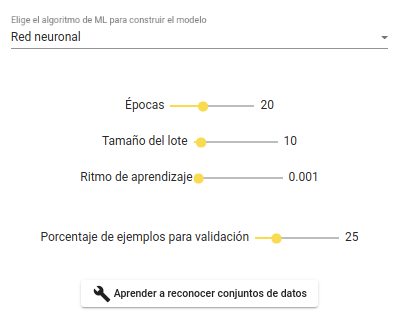
\includegraphics[width=9cm, keepaspectratio]{img/ej_num_rn.png}
	\caption{Configuración redes neuronales} 	\label{fig:ejemplo4}
\end{figure}

\begin{figure}
	\centering
	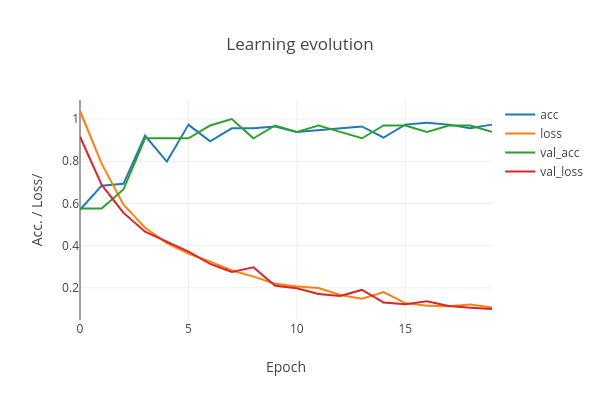
\includegraphics[width=10cm, keepaspectratio]{img/le_num_rn.png}
	\caption{Gráfica de evolución de aprendizaje redes neuronales con datos numéricos} 	\label{fig:ejemplo5}
\end{figure}

\begin{figure}
	\centering
	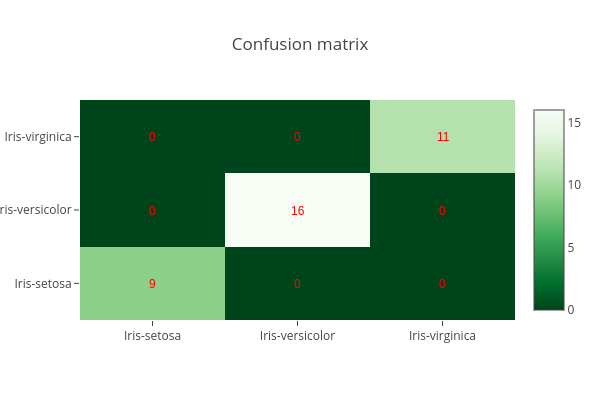
\includegraphics[width=12cm, keepaspectratio]{img/cm_num_rn.png}
	\caption{Matriz de confusión redes neuronales con datos numéricos. 25\% ejemplos de validación} 	
	\label{fig:ejemplo6}
\end{figure}

Una vez se ha comprobado la validez del modelo, se realizan pruebas en la aplicación con ejemplos de muestras en la parte de evaluación, para comprobar si realmente clasifica correctamente la muestra introducida. 

Para realizar las pruebas, se escogen tres muestras aleatorias del conjunto de datos, una de cada clase:
\begin{itemize}

\item[•] Se escoge una muestra de la clase iris setosa, se introduce en la parte de evaluación y como resultado se ve qué clase se le asigna. En la figura~\ref{fig:ejemplo7} se puede observar el porcentaje de que la muestra evaluada pertenezca a una clase u otra. En este caso asigna correctamente la muestra a la clase que le corresponde, ya que indica que al 99.5\% pertenece a la clase iris setosa. 

\item[•] Se escoge una muestra de la clase iris virginica. En este caso asigna correctamente la muestra a la clase que le corresponde, ya que indica que al 96.55\% pertenece a la clase iris virginica como se puede observar en la figura~\ref{fig:ejemplo8}.

\item[•] Se escoge una muestra de la clase iris versicolor. En este caso asigna correctamente la muestra a la clase que le corresponde, ya que indica que al 96.71\% pertenece a la clase iris versicolor como se puede observar en la figura~\ref{fig:ejemplo9}.
\end{itemize}

\begin{figure}
	\centering
	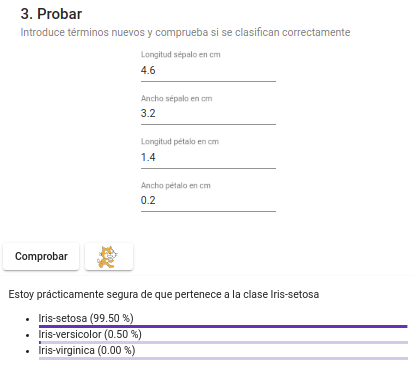
\includegraphics[width=9cm, keepaspectratio]{img/iris_set_num_rn.png}
	\caption{Muestra de test de la clase iris setosa con redes neuronales} 	\label{fig:ejemplo7}
\end{figure}

\begin{figure}
	\centering
	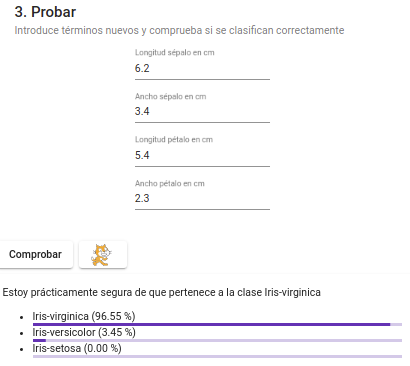
\includegraphics[width=9cm, keepaspectratio]{img/iris_vir_num_rn.png}
	\caption{Muestra de test de la clase iris virginica con redes neuronales} 	\label{fig:ejemplo8}
\end{figure}

\begin{figure}
	\centering
	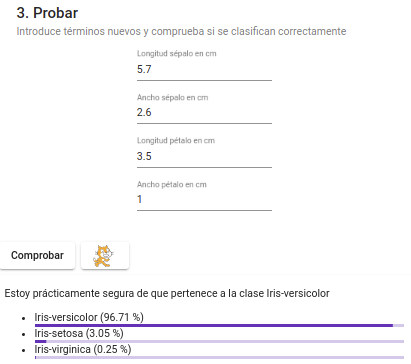
\includegraphics[width=9cm, keepaspectratio]{img/iris_ver_num_rn.png}
	\caption{Muestra de test de la clase iris versicolor con redes neuronales} 	\label{fig:ejemplo9}
\end{figure}

Se realizan además varias comprobaciones más con muestras de las tres clases y el algoritmo las clasifica correctamente. Pero en la figura~\ref{fig:ejemplo8}, que corresponde con la clase iris virginica, se puede ver que un pequeño porcentaje lo asigna a la clase iris versicolor, y en la figura~\ref{fig:ejemplo9}, que corresponde con la clase iris versicolor, se puede ver que un pequeño porcentaje lo asigna a la clase iris virginica. Esto sucede porque estas dos clases tienen características similares, en la figura~\ref{fig:flores-iris} se puede observar que la flor iris virginica y la flor iris versicolor son prácticamente iguales, y en algún caso puede tener un error de clasificación. Esto se puede comprobar viendo la matriz de confusión de la figura~\ref{fig:ejemplo10} en la que el porcentaje de ejemplos de validación se aumenta al 75\% para comprobar la validez con la mayoría de muestras. 
Aun así el porcentaje de acierto es muy alto. En este caso es del 96.36\%, ya que falla en la clasificación de cuatro muestras de un total de 110 muestras. Con esto se podría decir que el modelo funciona correctamente.
\begin{figure}
	\centering
	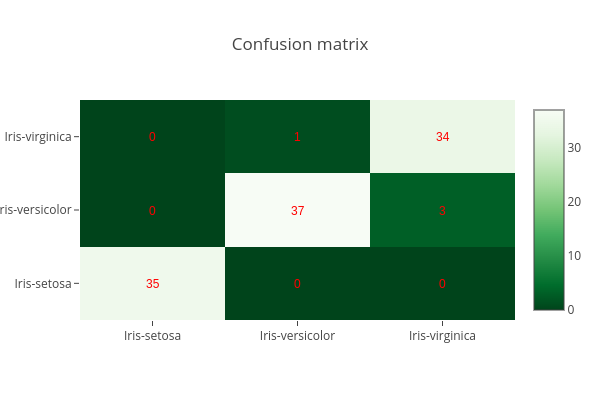
\includegraphics[width=12cm, keepaspectratio]{img/cm_num_rn2.png}
	\caption{Matriz de confusión redes neuronales con datos numéricos. 75\% ejemplos de validación} 	
	\label{fig:ejemplo10}
\end{figure}

\subsection{KNN}
\label{subsec:knn}

Para utilizar KNN se elige el clasificador de KNN en el desplegable, se selecciona el número de vecinos (en este caso lo dejamos como viene) y se escoge el porcentaje de muestras se usan como ejemplos de validación (en este caso seleccionamos un 25\%). La configuración resultante se puede observar en la figura~\ref{fig:ejemplo11}.

Con este algoritmo se puede comprobar la validez del modelo con la matriz de confusión. En la figura~\ref{fig:ejemplo12} se puede ver un ejemplo de la matriz de confusión, que en este caso tiene un 94.44\% de acierto, ya que falla en la clasificación de dos muestras de un total de 36 muestras. Se comprueba la matriz de confusión varias veces para que escoja diferentes muestras y el porcentaje de acierto es alto, ya que suele ser superior al 90\% por lo que se puede considerar un porcentaje de acierto bueno. El uso de este conjunto de datos no es común para el algoritmo KNN, pero con los resultados de la matriz de confusión se puede decir que su uso es apto y que las muestras se están recogiendo de la forma correcta.

\begin{figure}
	\centering
	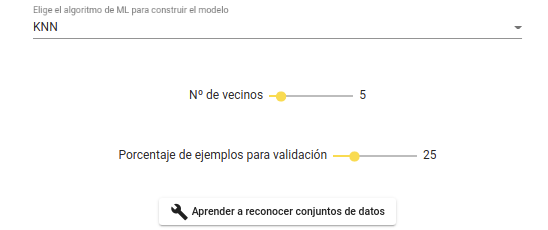
\includegraphics[width=9cm, keepaspectratio]{img/ej_num_knn.png}
	\caption{Configuración KNN} 	\label{fig:ejemplo11}
\end{figure}

\begin{figure}
	\centering
	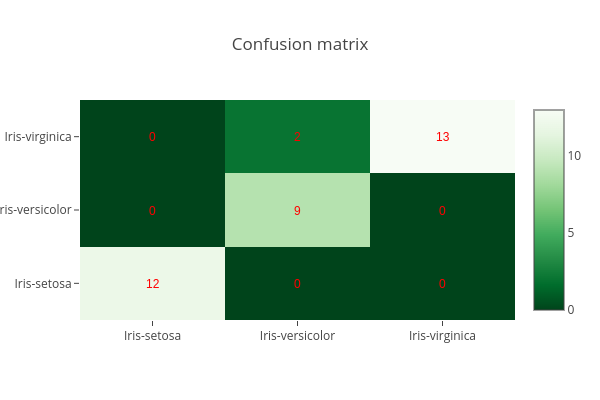
\includegraphics[width=12cm, keepaspectratio]{img/cm_num_knn.png}
	\caption{Matriz de confusión KNN con datos numéricos. 25\% ejemplos de validación} 	
	\label{fig:ejemplo12}
\end{figure}

Una vez se ha comprobado la validez del modelo, se realizan pruebas en la aplicación con ejemplos de muestras en la parte de evaluación para comprobar si realmente clasifica correctamente la muestra introducida, al igual que se hizo con redes neuronales.

Para realizar las pruebas, se escogen tres muestras aleatorias del conjunto de datos, una de cada clase:

\begin{itemize}
\item[•] Se escoge una muestra de la clase iris setosa. En este caso asigna correctamente la muestra a la clase que le corresponde, ya que indica que al 100\% pertenece a la clase iris setosa, como se puede observar en la figura~\ref{fig:ejemplo13}.

\item[•] Se escoge una muestra de la clase iris virginica. En este caso asigna correctamente la muestra a la clase que le corresponde, ya que indica que al 80\% pertenece a la clase iris virginica, como se puede observar en la figura~\ref{fig:ejemplo14}.

\item[•] Se escoge una muestra de la clase iris versicolor. En este caso asigna correctamente la muestra a la clase que le corresponde, ya que indica que al 80\% pertenece a la clase iris versicolor, como se puede observar en la figura~\ref{fig:ejemplo15}.
\end{itemize}

\begin{figure}
	\centering
	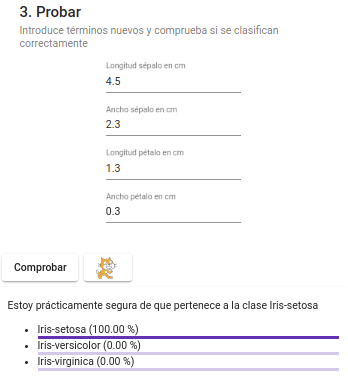
\includegraphics[width=9cm, keepaspectratio]{img/iris_set_num_knn.png}
	\caption{Muestra de test de la clase iris setosa con KNN} 	\label{fig:ejemplo13}
\end{figure}

\begin{figure}
	\centering
	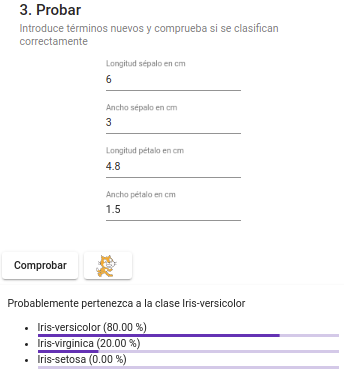
\includegraphics[width=9cm, keepaspectratio]{img/iris_vir_num_knn.png}
	\caption{Muestra de test de la clase iris virginica con KNN} 	\label{fig:ejemplo14}
\end{figure}

\begin{figure}
	\centering
	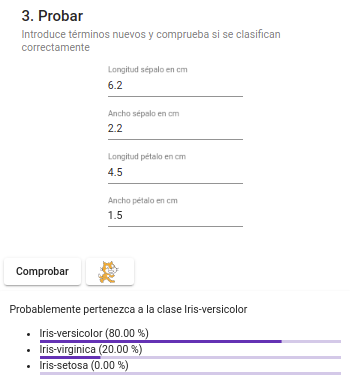
\includegraphics[width=9cm, keepaspectratio]{img/iris_ver_num_knn.png}
	\caption{Muestra de test de la clase iris versicolor con KNN} 	\label{fig:ejemplo15}
\end{figure}

En este caso los porcentajes son múltiplos de 20 debido a que el parámetro K (número de vecinos) tiene el valor 5, por lo que la muestra tendrá 1, 2, 3, 4 o 5 vecinos de una clase que se corresponden con el 20, 40, 60, 80 o 100 por ciento respectivamente. 
Este conjunto de datos no está pensado para su uso con este algoritmo porque como las clases iris virginica e iris versicolor tienen características similares, se colocan cerca las dos clases en la distribución que hace KNN de las muestras. Debido a esto, al escoger los vecinos más cercanos puede haber un fallo de asignación de la clase que es realmente. 
Aun así, se realizan varias comprobaciones más con muestras de las tres clases y el algoritmo las clasifica correctamente exceptuando algún fallo con estas dos clases. Esto se puede comprobar en la matriz de confusión de la figura~\ref{fig:ejemplo16} en la que el porcentaje de ejemplos de validación se aumenta al 75\% para comprobar la validez con la mayoría de muestras. 
Aun así, el porcentaje de acierto es muy alto, en este caso es del 94.5\%, ya que falla en la clasificación de seis muestras de un total de 110 muestras. Con esto se podría decir que el modelo funciona correctamente.

\begin{figure}
	\centering
	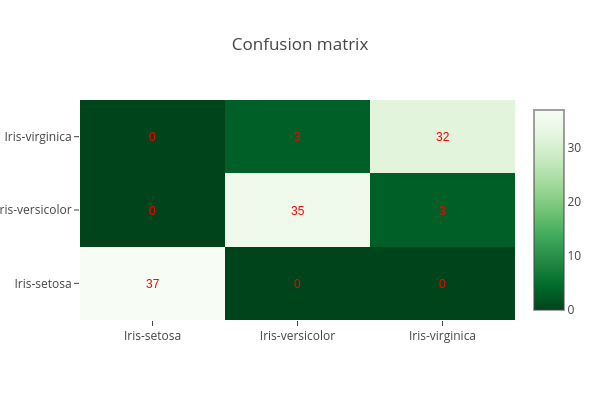
\includegraphics[width=12cm, keepaspectratio]{img/cm_num_knn2.png}
	\caption{Matriz de confusión KNN con datos numéricos. 75\% ejemplos de validación} 	
	\label{fig:ejemplo16}
\end{figure}

Con estos resultados obtenidos se puede decir que el modelo se crea correctamente con conjuntos de datos numéricos y que el conjunto de datos flor iris es válido para los dos tipos de algoritmos.

\section{Conjunto de datos numéricos y categóricos}
\label{subsec:numericosycategoricos}

Para comprobar la clasificación de un conjunto de datos numéricos y categóricos hemos utilizado el conjunto de datos de evaluación del coche que se encuentra en el archivo \texttt{car.json} de la carpeta datasets. Este dataset está compuesto de dos clases (good y vgood). La clase good tiene 69 muestras y la clase vgood tiene 65 muestras.
Los atributos de las muestras son precio de compra, precio de mantenimiento, número de puertas, capacidad de personas, tamaño del maletero y seguridad estimada. 
En la figura~\ref{fig:ejemplo17} se pueden observar las muestras de las distintas clases.

\begin{figure}
	\centering
	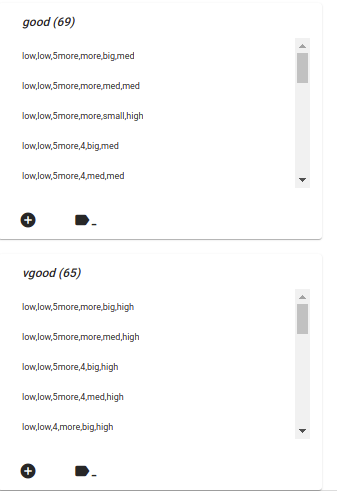
\includegraphics[width=9cm, keepaspectratio]{img/ejemplo_muestras_numycat.png}
	\caption{Muestras con datos numéricos para el entrenamiento} 	\label{fig:ejemplo17}
\end{figure}

Al igual que con el conjunto de datos numéricos se prueba la validez con el algoritmo de redes neuronales y con el algoritmo de KNN.

\subsection{Redes neuronales}
\label{subsec:redesneuronales}

Para utilizar redes neuronales la configuración es igual que en el caso de datos numéricos, como se puede ver en la figura~\ref{fig:ejemplo4}.
Hay dos formas de comprobar la validez del modelo con el algoritmo de redes neuronales:

\begin{enumerate}
\item Con la gráfica de evolución de aprendizaje. En la figura~\ref{fig:ejemplo18} se puede ver que cuantas más épocas pasan, más aciertos hay. Al final de la gráfica el acierto es casi 1 como pasa con el conjunto de datos numéricos.
Este resultado indica que el aprendizaje se está realizando correctamente.
 \item Con la matriz de confusión. En la figura~\ref{fig:ejemplo19} se puede ver un ejemplo de la matriz de confusión que en este caso tiene un 97\% de acierto, ya que falla en la clasificación de una muestra de un total de 33 muestras. Se comprueba la matriz de confusión varias veces y el fallo es muy bajo. El acierto suele ser superior al 90\% como pasa con el conjunto de datos numéricos, por lo que se puede considerar un porcentaje de acierto bueno.
 \end{enumerate}
 
 \begin{figure}
	\centering
	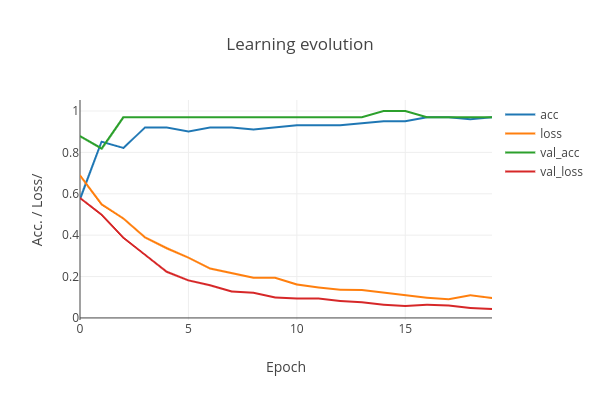
\includegraphics[width=10cm, keepaspectratio]{img/le_numycat_rn.png}
	\caption{Gráfica de evolución de aprendizaje redes neuronales con datos numéricos y categóricos} 	\label{fig:ejemplo18}
\end{figure}

\begin{figure}
	\centering
	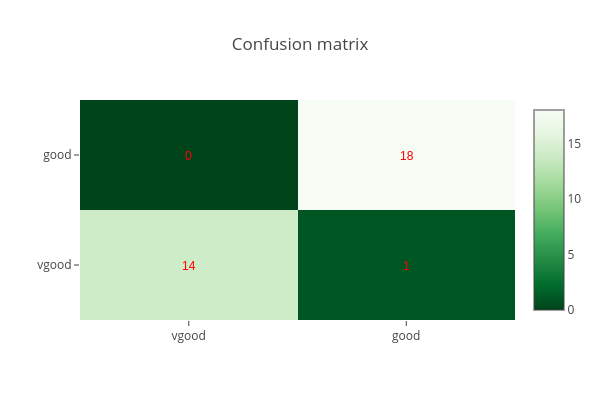
\includegraphics[width=12cm, keepaspectratio]{img/cm_numycat_rn.png}
	\caption{Matriz de confusión redes neuronales con datos numéricos y categóricos. 25\% ejemplos de validación} 	
	\label{fig:ejemplo19}
\end{figure}

 
Con los datos obtenidos en la gráfica de evolución de aprendizaje, figura~\ref{fig:ejemplo18}, y en la matriz de confusión, figura~\ref{fig:ejemplo19}, se puede decir que el modelo se crea correctamente. Esto implica que las muestras se recogen de forma correcta y que la extracción de características es correcta. Además, el algoritmo de redes neuronales es apto para el reconocimiento de este conjunto de datos.

Una vez se ha comprobado la validez del modelo, se realizan pruebas en la aplicación para comprobar si realmente clasifica correctamente la muestra introducida. Para ello se escogen dos muestras aleatorias del conjunto de datos, una de cada clase:

\begin{itemize}
\item[•] Se escoge una muestra de la clase good. En este caso asigna correctamente la muestra a la clase que le corresponde, ya que indica que al 86.54\% pertenece a la clase good, como se puede observar en la figura~\ref{fig:ejemplo20}.
\item[•] Se escoge una muestra de la clase vgood. En este caso asigna correctamente la muestra a la clase que le corresponde, ya que indica que al 95.13\% pertenece a la clase vgood, como se puede observar en la figura~\ref{fig:ejemplo21}. 
\end{itemize}

\begin{figure}
	\centering
	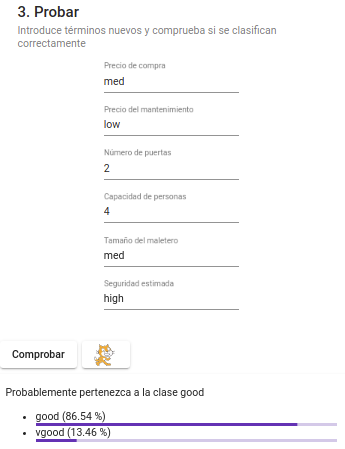
\includegraphics[width=9cm, keepaspectratio]{img/good_rn.png}
	\caption{Muestra de test de la clase good con redes neuronales} 	\label{fig:ejemplo20}
\end{figure}

\begin{figure}
	\centering
	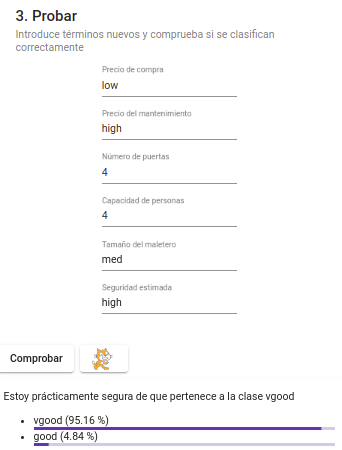
\includegraphics[width=9cm, keepaspectratio]{img/vgood_rn.png}
	\caption{Muestra de test de la clase vgood con redes neuronales} 	
	\label{fig:ejemplo21}
\end{figure}

Además, se realizan varias comprobaciones más con muestras de las dos clases y el algoritmo las clasifica correctamente. 
En algún caso puede fallar, ya que las características son similares entre las dos clases, pero el porcentaje de acierto es alto, como se puede comprobar en la matriz de confusión de la figura~\ref{fig:ejemplo22} en la que el porcentaje de ejemplos de validación se aumenta al 75\% para comprobar la validez con la mayoría de muestras. En este caso el porcentaje de acierto es del 88.7\%. Con estos resultados se podría decir que el modelo funciona correctamente.

\begin{figure}
	\centering
	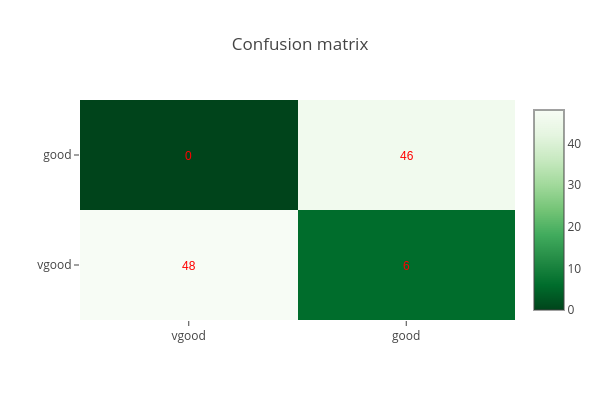
\includegraphics[width=12cm, keepaspectratio]{img/cm_numycat_rn2.png}
	\caption{Matriz de confusión redes neuronales con datos numéricos y categóricos. 75\% ejemplos de validación} 	
	\label{fig:ejemplo22}
\end{figure}

\subsection{KNN}
\label{subsec:knn}

Para hacer uso de KNN la configuración es igual que en el caso de datos numéricos, como se muestra en la figura~\ref{fig:ejemplo11}. Con este algoritmo se puede comprobar la validez del modelo con la matriz de confusión. En la figura~\ref{fig:ejemplo23} se puede ver un ejemplo de la matriz de confusión que en este caso tiene un 94.28\% de acierto, ya que falla en la clasificación de dos muestras de un total de 35 muestras. Se comprueba la matriz de confusión varias veces para que escoja diferentes muestras y el porcentaje de acierto es alto. Suele ser superior al 80\% por lo que se puede considerar un porcentaje de acierto bueno. Se podría decir que el modelo se crea correctamente.

\begin{figure}
	\centering
	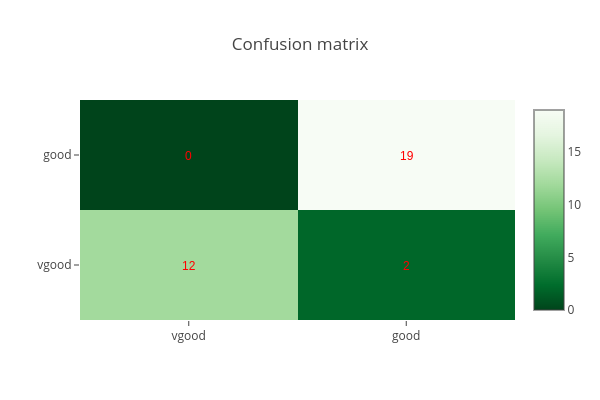
\includegraphics[width=12cm, keepaspectratio]{img/cm_numycat_knn.png}
	\caption{Matriz de confusión KNN con datos numéricos y categóricos. 25\% ejemplos de validación} 	
	\label{fig:ejemplo23}
\end{figure}

Una vez se ha comprobado la validez del modelo, se realizan pruebas en la aplicación con ejemplos de muestras en la parte de evaluación para comprobar si realmente clasifica correctamente la muestra introducida, al igual que se hizo con redes neuronales.

Para realizar las pruebas se escogen dos muestras aleatorias del conjunto de datos, una de cada clase:

\begin{itemize}
\item[•] Se escoge una muestra de la clase good. En este caso asigna correctamente la muestra a la clase que le corresponde, ya que indica que al 100\% pertenece a la clase good, como se puede observar en la figura~\ref{fig:ejemplo24}.
\item[•] Se escoge una muestra de la clase vgood. En este caso asigna correctamente la muestra a la clase que le corresponde, ya que indica que al 100\% pertenece a la clase vgood, como se puede observar en la figura~\ref{fig:ejemplo25}.
\end{itemize}

\begin{figure}
	\centering
	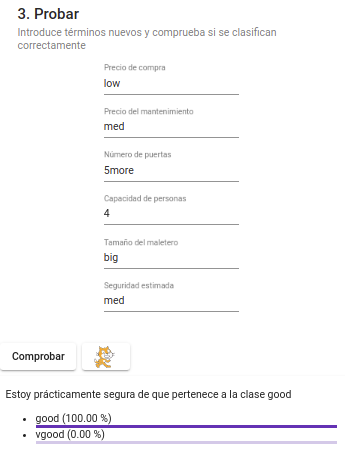
\includegraphics[width=9cm, keepaspectratio]{img/good_knn.png}
	\caption{Muestra de test de la clase good con KNN} 	\label{fig:ejemplo24}
\end{figure}

\begin{figure}
	\centering
	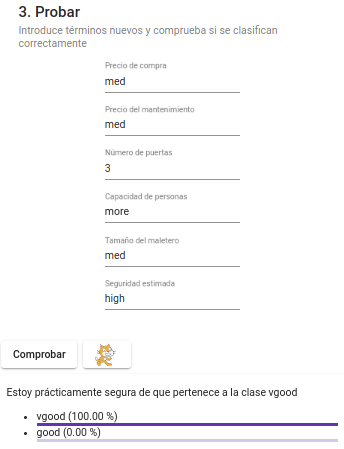
\includegraphics[width=9cm, keepaspectratio]{img/vgood_knn.png}
	\caption{Muestra de test de la clase vgood con KNN} 	\label{fig:ejemplo25}
\end{figure}

Además, se realizan varias comprobaciones más con muestras de las dos clases y el algoritmo las clasifica correctamente exceptuando algún fallo. Esto se puede comprobar en la matriz de confusión de la figura~\ref{fig:ejemplo26} en la que el porcentaje de ejemplos de validación se aumenta al 75\% para comprobar la validez con la mayoría de muestras. 
Aun así, el porcentaje de acierto es aceptable. En este caso es del 69\%, ya que falla en la clasificación de 31 muestras de un total de 100 muestras. Con esto se podría decir que el modelo funciona correctamente, pero que el uso de este algoritmo no es el más adecuado.

\begin{figure}
	\centering
	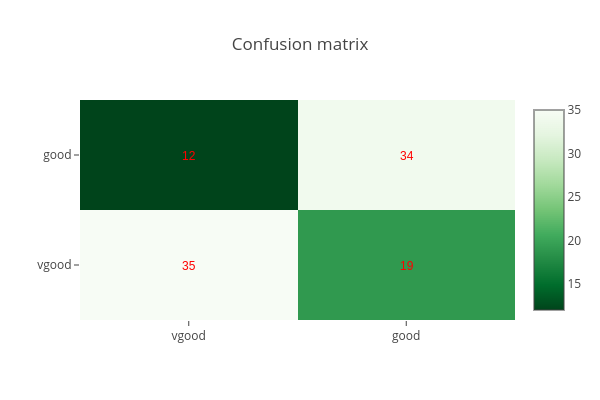
\includegraphics[width=12cm, keepaspectratio]{img/cm_numycat_knn2.png}
	\caption{Matriz de confusión KNN con datos numéricos y categóricos. 75\% ejemplos de validación} 	
	\label{fig:ejemplo26}
\end{figure}

Con estos resultados obtenidos se puede decir que el modelo se crea correctamente con conjuntos de datos numéricos y categóricos y que el conjunto de datos de evaluación de coche es válido para los dos tipos de algoritmos, pero es mejor usarlo con el algoritmo de redes neuronales.

Como resultado final se puede decir que la creación de modelos de conjuntos de datos es válida, es decir, las muestras se recogen correctamente y la extracción de características también es correcta ya sea con datos numéricos o categóricos, y que dependiendo de como sean los conjuntos de datos funcionará mejor un algoritmo u otro.




%%%%%%%%%%%%%%%%%%%%%%%%%%%%%%%%%%%%%%%%%%%%%%%%%%%%%%%%%%%%%%%%%%%%%%%%%%%%%%%%
%%%%%%%%%%%%%%%%%%%%%%%%%%%%%%%%%%%%%%%%%%%%%%%%%%%%%%%%%%%%%%%%%%%%%%%%%%%%%%%%
% CONCLUSIONES %
%%%%%%%%%%%%%%%%%%%%%%%%%%%%%%%%%%%%%%%%%%%%%%%%%%%%%%%%%%%%%%%%%%%%%%%%%%%%%%%%

\cleardoublepage
\chapter{Conclusiones}
\label{chap:conclusiones}

Consideramos que el resultado del trabajo ha sido bueno y creemos que la implementación de esta funcionalidad era necesaria para \texttt{LearningML}, ya que los conjuntos de datos están a la orden del día y los alumnos deben conocer qué son y la utilidad que pueden tener. En esto coincide Juan David Rodríguez, el co-tutor y desarrollador principal de \texttt{LearningML}, que quedó muy satisfecho con el trabajo realizado.


\section{Consecución de objetivos}
\label{sec:consecucion-objetivos}

Haciendo referencia al capítulo 2, el objetivo principal del TFG era implementar la nueva funcionalidad para reconocer conjuntos de datos. Este objetivo se ha cumplido como se esperaba.

En cuanto a los objetivos específicos, también se han cumplido. La arquitectura de \texttt{LearningML} la hemos entendido y hemos seguido la dinámica de lo ya creado. Se ha modificado la interfaz correctamente y la creación de conjuntos de datos se realiza correctamente y de una forma sencilla e intuitiva. Por último, la extracción de características se realiza correctamente y los resultados obtenidos son buenos.

\section{Aplicación de lo aprendido}
\label{sec:aplicacion}

Para la realización del proyecto, se han usado los conocimientos de varias asignaturas cursadas durante el grado como son las siguientes:

\begin{enumerate}
  \item[•] \textbf{Construcción de Servicios y Aplicaciones Audiovisuales en Internet (\emph{CSAAI})}. Esta asignatura ha sido de gran ayuda para tener conocimientos sobre el desarrollo web con lenguajes como JavaScript, HTML5 y CSS.
  
  \item[•] \textbf{Laboratorio de Tecnologías Audiovisuales en la Web (\emph{LTAW})}. Esta asignatura ha sido de gran ayuda para tener conocimientos sobre el desarrollo de aplicaciones web, ya que aprendes a usar Node.js y plantillas.
  
  \item[•] \textbf{Informática II}. Es una asignatura en la que aprendes un lenguaje complicado y altamente tipado como Ada, en el que aprendes a como llevar a cabo un programa de forma eficiente y limpia.
  
  \item[•] \textbf{Tratamiento Digital de la Imagen y Tratamiento Digital del Sonido}. Esta asignatura ha sido de gran ayuda para comprender como funcionan los algoritmos utilizados en \texttt{LearningML}.
  
  \item[•] \textbf{Protocolos para la Transmisión de Audio y Vídeo por Internet (\emph{PTAVI})}. Esta asignatura es la que realmente hizo que cogiera el gusto a programar y en la que entendí cómo funcionaba la programación.
  
\end{enumerate}


\section{Lecciones aprendidas}
\label{sec:lecciones_aprendidas}

Con la implementación de la nueva funcionalidad hemos ampliado y mejorado los conocimientos adquiridos durante la carrera en el desarrollo de aplicaciones web además de aprender otros nuevos como son:

\begin{enumerate}
  \item Angular. Al principio tuvimos que dedicar bastante tiempo a entender su funcionamiento, pero nos ha parecido muy útil porque facilita mucho el desarrollo web y de una forma muy organizada sobre todo para aplicaciones grandes debido a su arquitectura de componentes, servicios y módulos permite separar las funcionalidades y que se repita el código. Gracias a este framework, añadir una nueva funcionalidad ha sido más sencillo y nos alegramos de haber aprendido a usar este framework porque tiene un gran potencial.
  
  \item Programación asíncrona. Antes de empezar el proyecto teníamos una noción básica de que era la programación asíncrona, pero no sabía para qué podría usarse ni cómo implementarla. Una vez realizado el proyecto creemos que es muy útil e indispensable en ciertas acciones de una aplicación web, porque que no se bloquee es algo que valora mucho el usuario.
  
  \item TypeScript. No nos resultó difícil comprender este lenguaje, debido a que está basado en JavaScript, pero con cambios que son sencillos de entender. Es un lenguaje que me parece más útil que JavaScript, ya que tiene sus cosas buenas y fortalece sus debilidades.
\end{enumerate}


\section{Trabajos futuros}
\label{sec:trabajos_futuros}

Las mejoras que se pueden añadir a la aplicación web \texttt{LearningML} pueden ser:

\begin{itemize}
 \item[•] Se podría mejorar la creación del conjunto de datos creando un componenete nuevo. Con este componente se crearía una nueva página, en la que se crea el conjunto de datos en forma de tabla directamente y una vez se guarde, vuelva a \texttt{ml-model}. El conjunto de datos se mostraría igual que ahora en \texttt{ml-label-container}. Pero para modificar o añadir el conjunto de datos se haría en el nuevo componente.
 
 \item[•] Se podría añadir un boton de información en el que se explique que son los conjuntos de datos y un enlace a una página donde se puedan obtener conjuntos de datos.
 
 \item[•] Desarrollar una versión offline del editor de LML y de Scratch.
 
 \item[•] Añadir una nueva funcionalidad para el reconocimiento de la postura de la mano o de poses.
 
 \item[•] Incluir otros algoritmos de aprendizaje como puede ser las máquinas de vectores de soporte.
 \end{itemize} 


%%%%%%%%%%%%%%%%%%%%%%%%%%%%%%%%%%%%%%%%%%%%%%%%%%%%%%%%%%%%%%%%%%%%%%%%%%%%%%%%
%%%%%%%%%%%%%%%%%%%%%%%%%%%%%%%%%%%%%%%%%%%%%%%%%%%%%%%%%%%%%%%%%%%%%%%%%%%%%%%%
% BIBLIOGRAFIA %
%%%%%%%%%%%%%%%%%%%%%%%%%%%%%%%%%%%%%%%%%%%%%%%%%%%%%%%%%%%%%%%%%%%%%%%%%%%%%%%%

\cleardoublepage

% Las siguientes dos instrucciones es todo lo que necesitas
% para incluir las citas en la memoria
\bibliographystyle{abbrv}
\bibliography{memoria}  % memoria.bib es el nombre del fichero que contiene
% las referencias bibliográficas. Abre ese fichero y mira el formato que tiene,
% que se conoce como BibTeX. Hay muchos sitios que exportan referencias en
% formato BibTeX. Prueba a buscar en http://scholar.google.com por referencias
% y verás que lo puedes hacer de manera sencilla.
% Más información: 
% http://texblog.org/2014/04/22/using-google-scholar-to-download-bibtex-citations/

\end{document}
